% 2018.01.08 Modified
% 2015.07.10 Modified
%
% mthesis.tex
%
\documentclass[12pt]{jarticle} % Japanese
\usepackage{comment}
\usepackage[dvipdfmx]{graphicx}
\usepackage{ascmac}
\usepackage[table,xcdraw]{xcolor}
\usepackage{eclbkbox}
\usepackage{amsmath}
\usepackage{url}



%\documentclass[12pt]{article} % English
% if there are problems in the above regarding fonts, use this
% \documentclass[UTF8]{ctexart}

\usepackage[utf8]{inputenc}
%\usepackage{utf}
\usepackage{naist-jmthesis} %Japanese
%\usepackage{naist-mthesis} %English

\usepackage{graphicx}

%
% Page style
%
\pagestyle{final}       % Camera-Ready
%\pagestyle{draft}      % Draft
%
%
\lang{Japanese} % Japanese
%\lang{English} % English
%
% Student Number
%
\studentnumber{1811098}
%
% 修士論文 か 課題研究 かの選択
%
\doctitle{\mastersthesis}       % 修士論文
%\doctitle{\mastersreport}      % 課題研究
%
% 取得予定の修士号は 修士(工学) か 修士(理学) か ?
%
\major{\engineering}    % 工学
%\major{\science}       % 理学
%
% 日本語題目 (in LaTeX)
%
\title{ソースコードの類似性に基づいたテストコード\\自動推薦ツールSuiteRec}
%
% 日本語題目 (in plain text)
%
%   注: (in LaTeX)と同じ場合は指定する必要なし。
%       この情報は修士論文/課題研究には現れませんが、管理のために必要です。
%
\ptitle{ソースコードの類似性に基づいたテストコード\\自動推薦ツールSuiteRec}
%
% 英語題目 (in LaTeX)
%
\etitle{Automatic Test Suite Recommendation System based on Code Clone Detection}
%
% 英語題目 (in plain text)
%
%   注: (in LaTeX)と同じ場合は指定する必要なし。
%       この情報は修士論文/課題研究には現れませんが、管理のために必要です。
%
\eptitle{Automatic Test Suite Recommendation System based on Code Clone Detection}
%
% 日本語氏名 (in LaTeX)
%   (姓と名の間に空白を入れて下さい)
%
\author{倉地 亮介}
%
% 日本語氏名 (in plain text)
%
%   注: (in LaTeX)と同じ場合は指定する必要なし。
%       この情報は修士論文/課題研究には現れませんが、管理のために必要です。
%
\pauthor{}
%
% 欧文氏名 (in LaTeX)
%   (first name, last name の順に記入し、先頭文字のみを大文字にする。)
%
\eauthor{Ryosuke Kurachi}
% 別の例: \eauthor{Kurt G\"{o}del}
%
%
% 欧文氏名 (in plain text)
%
%   注: (in LaTeX)と同じ場合は指定する必要なし。
%       この情報は修士論文/課題研究には現れませんが、管理のために必要です。
%
\epauthor{}
% 別の例: \peauthor{Kurt Goedel}
%
%
% 論文提出年月日
%
\syear{2020}
\smonth{1}
\sday{28}
%
% 専攻の選択
%
\department{\infproc}  % 情報処理学
%\department{\infsys}    % 情報システム学
%\department{\bioinf}   % 情報生命科学
%\department{\infsci}    % 情報科学
%
%
% 審査委員(日本語)
%   (姓と名、名と称号の間に空白を入れて下さい)
%
%5人以上の場合,5人目以降は\addcmembers を使って宣言する。
%最大で合わせて8人まで宣言可能。
%主指導教員、副指導教員を明記する。両指導教員以外は委員。
%学外審査委員は、大学名を明記する
%
% 4人の場合
\cmembers{飯田 元 教授}{(主指導教員)}
         {井上 美智子 教授}{(副指導教員)}
         {市川 昊平 准教授}{(副指導教員)}
         {崔 恩瀞 准教授}{(京都工芸繊維大学)}
%
% 3人の場合
%\cmembers{○○ ○○ 教授}{(主指導教員)}
%         {○○ ○○ 教授}{(副指導教員)}
%         {○○ ○○ 准教授}{(副指導教員)}
%         {}{}
%
% 2人の場合
%\cmembers{○○ ○○ 教授}{(主指導教員)}
%         {○○ ○○ 教授}{(副指導教員)}
%          {}{}
%          {}{}
%
% 5人目の宣言
%\addcmembers{55 55 准教授}{(□□大学)}
%            {}{}
%            {}{}
%            {}{}
%
% 5〜6人目の宣言
%\addcmembers{55 55 准教授}{(□□大学)}
%            {66 66 准教授}{(□□大学)}
%            {}{}
%            {}{}
%
% 5〜7人目の宣言
%\addcmembers{55 55 准教授}{(□□大学)}
%            {66 66 准教授}{(□□大学)}
%            {77 77 准教授}{(□□大学)}
%            {}{}
%
% 5〜8人目の宣言
%\addcmembers{55 55 准教授}{(□□大学)}
%            {66 66 准教授}{(□□大学)}
%            {77 77 准教授}{(□□大学)}
%            {88 88 准教授}{(□□大学)}
%
%
% 審査委員(英語)
%     (first name, last name の順に記入し、先頭文字のみを大文字にする。
%       first name と last name の間に空白、
%       last name と 称号の間にカンマと空白を入れて下さい。)
%
% 5人以上の場合,5人目以降は\eaddcmembers を使って宣言する
% Supervisor, Co-supervisor, and Member must be specified.
% 4人の場合
\ecmembers{Professor XXX XXX}{(Supervisor)}
          {Professor XXX XXX}{(Co-supervisor)}
          {Associate Professor XXX XXX}{(Co-supervisor)}
          {Associate Professor XXX XXX}{(YY University)}
%
% 3人の場合
%\ecmembers{Professor XXX XXX}{(Supervisor)}
%          {Professor XXX XXX}{(Co-supervisor)}
%          {Associate Professor XXX XXX}{(Co-supervisor)}
%          {}{}
%
% 2人の場合
% \ecmembers{Professor XXX XXX}{(Supervisor)}
%           {Professor XXX XXX}{(Co-supervisor)}
%           {}{}
%           {}{}
%
% 5人目の宣言
%\eaddcmembers{Professor 55 55}{(YY University)}
%            {}{}
%            {}{}
%            {}{}
%
% 5〜6人目の宣言
%\eaddcmembers{Professor 55 55}{(YY University)}
%             {Professor 66 66}{(YY University)}
%             {}{}
%             {}{}
%
% 5〜7人目の宣言
%\eaddcmembers{Professor 55 55}{(YY University)}
%             {Professor 66 66}{(YY University)}
%             {Professor 77 77}{(YY University)}
%             {}{}
%
% 5〜8人目の宣言
%\eaddcmembers{Professor 55 55}{(YY University)}
%             {Professor 66 66}{(YY University)}
%             {Professor 77 77}{(YY University)}
%             {Professor 88 88}{(YY University)}
%
%
%
% キーワード5〜6個 (in LaTeX)
%
\keywords{コードクローン検出,推薦システム,ソフトウェアテスト,テストスメル,単体テスト}
%
% キーワード5〜6個 (in plain text)
%
%   注: (in LaTeX)と同じ場合は記入する必要なし。
%       この情報は修士論文/課題研究には現れませんが、管理のために必要です。
%
\pkeywords{コードクローン検出,推薦システム,ソフトウェアテスト,テストスメル,単体テスト}
%
% 5 or 6 Keywords (in LaTeX)
%
\ekeywords{clone detection, recommendation system, software testing, test smell, unit test}
%
% 5 or 6 Keywords (in plain text)
%
%   注: (in LaTeX)と同じ場合は記入する必要なし。
%       この情報は修士論文/課題研究には現れませんが、管理のために必要です。
%
\epkeywords{clone detection, recommendation system, software testing, test smell, unit test}
%
% 内容梗概 (in LaTeX)
%
%   注: 行の先頭が\\で始まらないようにすること。
%
\abstract{
ソフトウェアの品質確保の要と言えるソフトウェアテストを支援することは,重要である.これまでにテスト作成コストを削減するために,様々な自動生成技術が提案されてきた.しかし,既存ツールによって自動生成されたテストコードは,テスト対象コードの作成経緯や意図に基づいて生成されていないという性質から保守作業を困難にさせる課題がある.この課題の解決方法として,既存テストの再利用が有効であると考えられる.本研究ではオープンソースソフトウェアに存在する品質が高いテストコードを推薦するツール{\sf SuiteRec}を提案する.{\sf SuiteRec}は,クローンペア間でのテスト再利用を考える.開発者からの入力コード片に対して類似コード片を検出し,その類似コード片に対応するテストスイートを推薦する.さらに,テストコードの良くない実装を表す指標であるテストスメルを開発者に提示し,より品質の高いテストスイートを推薦できるように推薦順位を並び替える.評価実験では,被験者によって{\sf SuiteRec}を使用した場合とそうでない場合でテストコードの作成してもらい,テスト作成をどの程度支援できるかを定量的および定性的に評価した.その結果,{\sf SuiteRec}を利用した場合,(1) 条件分岐が多いプログラムのテストコードを作成する際にコードカバレッジの向上に効果的であること,(2) 作成したテストコードはテストスメルの数が少なく品質が高いこと,(3) 開発者はテストコード作成作業を容易だと認識し,自身で作成したテストコードに自信が持てることが分かった.また,{\sf SuiteRec}は開発者が参考にしたいテストスイートを上位に推薦できることを確認した. 
}
%
% 内容梗概 (in plain text)
%
%   注: (in LaTeX)と同じ場合は記入する必要なし。
%       この情報は修士論文/課題研究には現れませんが、管理のために必要です。
%       改行する箇所には空白行を入れる。
%       行の先頭が\\で始まらないようにすること。
%
\pabstract{
ソフトウェアの品質確保の要と言えるソフトウェアテストを支援することは重要である.これまでにテスト作成コストを削減するために様々な自動生成技術が提案されてきた.しかし,既存ツールによって自動生成されたテストコードはテスト対象コードの作成経緯や意図に基づいて生成されていないという性質から後の保守活動を困難にさせる課題がある.この課題の解決方法として,既存テストの再利用が有効であると考えられる.本研究ではOSSプロジェクト上に存在する既存の品質が高いテストコードを推薦するツール{\sf SuiteRec}を提案する.{\sf SuiteRec}は,クローンペア間でのテスト再利用を考える.開発者からの入力コード片に対して類似コード片を検出し,その類似コード片に対応するテストスイートを推薦する.さらに,テストコードの良くない実装を表す指標であるテストスメルを開発者に提示し,より品質の高いテストスイートを推薦できるように推薦順位を並び替える.評価実験では,被験者によって{\sf SuiteRec}を使用した場合とそうでない場合でテストコードの作成してもらい,テスト作成をどの程度支援できるかを定量的および定性的に評価した.その結果,{\sf SuiteRec}を利用した場合,(1) 条件分岐が多いプログラムのテストコードを作成する際にコードカバレッジの向上に効果的であること,(2) 作成したテストコードはテストスメルの数が少なく品質が高いこと,(3) 開発者はテストコードの作成作業を容易だと認識し,自身で作成したテストコードに自信が持てることが分かった.また,{\sf SuiteRec}は開発者が参考にしたいテストスイートを上位に推薦できることを確認した. 
}
%
% Abstract (in LaTeX)
%
%  注:  行の先頭が\\で始まらないようにすること。
%
\eabstract{
Software testing is vital to ensure the quality of software. In previous studies, various techniques to automatically generate test codes have been proposed to reduce development costs. However, automatically generated tests tend to ignore the development process and intention behind the target code, and therefore generally considered to be less readable and maintainable. This places a question mark over their practical value. To solve this problem, we propose {\sf SuiteRec}, a recommendation tool to find existing high-quality test codes from OSS projects. The basic idea behind {\sf SuiteRec} is that test codes can be reused between code clone pairs. {\sf SuiteRec} finds code clones of the input code from OSS projects and recommends test suites corresponding to the clones. The recommended test suites are sorted by their quality and presented to the developer. Furthermore, test smells, which indicate bad implementation of test codes, are shown for each test suite. In the evaluation, we asked subjects to develop test codes with and without using {\sf SuiteRec} and compared the developed test codes. We show that (1) {\sf SuiteRec} improves code coverage when developing test codes for target codes with many conditional branches, (2) test codes created using {\sf SuiteRec} have higher quality and less test smells, and (3) developers feel that it is easier to develop test codes, and they are more confident in the resulting test codes when using {\sf SuiteRec}. In addition, we have confirmed that {\sf SuiteRec} can recommend test suites to the top rankings that developers want to refer.
}
%
% Abstract (in plain text)
%
%   注: (in LaTeX)と同じ場合は記入する必要なし。
%       この情報は修士論文/課題研究には現れませんが、管理のために必要です。
%       改行する箇所には空白行を入れる。
%       行の先頭が\\で始まらないようにすること。
%
\epabstract{
Automatically generated tests tend to be less read-able and maintainable since they often do not consider thelatent objective of the target code. Reusing existing tests mighthelp address this problem. To this end, we present SuiteRec, asystem that recommends reusable test suites based on code clonedetection. Given a java method, SuiteRec searches for its codeclones from a code base collected from open-source projects,and then recommends test suites of the clones. It also providesthe ranking of the recommended test suites computed basedon the similarity between the input code and the cloned code.We evaluate SuiteRec with a human study of ten students. Theresults indicate that SuiteRec successfully recommends reusabletest suites.
}
%%%%%%%%%%%%%%%%%%%%%%%%% document starts here %%%%%%%%%%%%%%%%%%%%%%%%%%%%
\begin{document}
%
% 表紙 および アブストラクト
%
\titlepage
\cmemberspage
\firstabstract
\secondabstract
%
% 目次
%
\toc
\newpage
\listoffigures
%\newpage
\listoftables
%
% これ以降本文
%
\newpage
\section{はじめに}
\pagenumbering{arabic}
近年,ソフトウェアに求められる要件が高度化・多様化する一方,ユーザからはソフトウェアの品質確保やコスト削減に対する要求も増加している\cite{tanno}.その中でもソフトウェア開発全体のコストに占める割合が大きく,品質確保の要ともいえるソフトウェアテストを支援する技術への関心が高まっている\cite{b20}.しかし,現状ではテスト作成作業の大部分が人手で行われており,多くのテストを作成しようとするとそれに比例してコストも増加してしまう.このような背景から,ソフトウェアの品質を確保しつつコスト削減を達成するために,様々な自動化技術が提案されている\cite{b19,EvoSuite,GRT,b17,T3}.

既存研究で提案されている{\sf EvoSuite}\cite{EvoSuite}は,単体テスト自動生成における最先端のツールである.{\sf EvoSuite}は,対象コードを静的解析しプログラムを記号値で表現する.そして,対象コードの制御パスを通るような条件を集め,条件を満たす具体値を生成する.単体テストを自動生成することで,開発者は手作業でのテスト作成時間が自動生成によって節約することができ,またコードカバレッジを大幅に向上することができる.しかし,既存ツールによって自動生成されるテストコードは対象のコードの作成経緯や意図に基づいて生成されていないという性質から保守作業を困難にするという課題がある\cite{b14,b15,b13}.これは,自動生成ツールの実用的な利用の価値に疑問を呈する.テストが失敗するたびに,開発者はテスト対象のコード内で不具合の原因を特定するまたは,テスト自体を更新するか否かを判断する必要がある.自動生成されたテストコードは読みづらく,開発者の助けになるというより,むしろ保守作業を困難にするという結果が報告されている\cite{b1}.従って,自動生成技術によって一時的に削減できたコストは,後の保守作業を通して返済される可能性がある.

我々は,この課題の解決するために既存テストの再利用が有効であると考える.本研究では,オープンソースソフトウェア(以下,OSS)に存在する既存の品質の高いテストコード推薦するツール{\sf SuiteRec}を提案する.推薦手法の基本となるアイディアはクローンペア間でのテストコード再利用である.{\sf SuiteRec}は,入力コード片に対して類似コード片を検出し,その類似コード片に対応するテストスイートを開発者に推薦する.さらに,テストコードの良くない実装を表す指標であるテストスメルを開発者に提示し,より品質の高いテストスイートを推薦できるように推薦順位がランキングされる.

評価実験では,被験者によって{\sf SuiteRec}の使用した場合とそうでない場合でテストコードの作成してもらい,テスト作成をどの程度支援できるかを定量的および定性的に評価した.その結果,{\sf SuiteRec}の利用は条件分岐が多く複雑なプログラムのテストコードを作成する際に,コードカバレッジの向上に効果的であること,作成したテストコードに含まれるテストスメルの数が少なく品質が高いことが分かった.また,{\sf SuiteRec}は開発者が参考にしたいテストコードを上位に推薦できることを確認した.実験後のアンケートによる定性的な評価では,{\sf SuiteRec}を使用した場合,被験者はテストコードの作成が容易になると認識し,また自分の作成したコードに自信が持てることが分かった.

以降,2章では,本研究に関わるコードクローン及びソフトウェアテストについての背景を説明する.3章では,本研究で提案するテストコード自動推薦ツール{\sf SuiteRec}ついて説明する.4章では,被験者による{\sf SuiteRec}の評価実験について説明する.5章では,{\sf SuiteRec}の有効性と妥当性への脅威について議論する.最後に6章で,まとめと今後の課題について説明する.

%\ref{kako}節では、過去における研究について述べ、
%\ref{kadai}章では、現状と今後の課題について述べる。
%また、付録\ref{omake1}におまけその1を添付する。

\newpage
\section{背景}
\subsection{コードクローン}

コードクローンとは,ソースコード中に存在する同一,あるいは類似した部分を持つコード片のことであり,コピーアンドペーストなどの様々な理由により生成される\cite{c1}.互いにコードクローンになるコード片の対のことをクローンペアと呼び,クローンペアにおいて推移関係が成り立つコードクローンの集合のことをクローンクラスと呼ぶ.これまでの研究\cite{c2,c3,c1}では,コードクローンの存在は,ソフトウェアの保守を困難にすると言われており除去すべきと考えられていた.しかし,最近の調査ではソフトウェアの開発・保守に影響を与えるのは一部のコードクローンだけであることが明らかになり,コードクローンを除去するのではなく活用した研究も多く提案されている.

\subsubsection{コードクローンの分類}
既存研究\cite{c5,c4}では,  クローンペア間の違いの度合いに基づき,コードクローンを以下の4種類に分類している.

\begin{itemize}
\item \textbf{タイプ1} : 空白やタブの有無,括弧の位置などのコーディングスタイル,コメントの有無などの違いを除き完全に一致するコードクローン
\item \textbf{タイプ2} : タイプ1のコードクローンの違い加えて,変数名や関数名などのユーザ定義名,変数の型などが異なるコードクローン
\item \textbf{タイプ3} : タイプ2のコードクローンの違いに加えて,文の挿入や削除,変更などが行われたコードクローン
\item \textbf{タイプ4} : 同一の処理を実行するが,構文上の実装が異なるコードクローン
\end{itemize}

\subsubsection{コードクローン検出技術}
これまでの研究において,様々なコードクローン検出技術が提案されてきた\cite{c6,c1}.本節では,代表的な3つの検出技術を紹介する.

\begin{description}
\item[文字/行単位の検出]~\\
この検出手法では,ソースコードを文字(または行)の並びで表現し,一定以上の長さで同じ文字(行)の並びが出現する部分をコードクローンとして検出する.他の検出技術に比べ検出速度が高速という利点があるが,文字列の並びを比較するため構文的に類似したコード片を検出するのが困難である.
\item[字句単位の検出]~\\
字句単位の検出手法では,検出の前処理としてソースコードを字句の列に変換する.そして,閾値以上の長さで一致している字句の部分列をコードクローンとして検出する.文字/行単位の検出に比べ,構文的に類似したコード片に対しても,ある程度柔軟に検出することができる.
\item[抽象構文木を用いた検出]~\\
抽象構文木とは,ソースコードの構文構造を木構造で表したグラフのことを意味する.この検出手法では,検出の前処理としてソースコードに対して構文解析を行うことによって,抽象構文木を構築する.そして,抽象構文木上の同型の部分木をコードクローンとして検出する.他の検出技術に比べ,部分木の同型判定を行うので計算コストが高くなる.
\end{description}

\subsection{ソフトウェアテスト}
ソフトウェアテスト(以下,テスト)とは,ソフトウェア開発プロセスの中で最後の品質を確保する工程である.テストは,ソフトウェアが仕様書通りに動作することを確認すること,また不具合を検出し修正することでソフトウェアの品質を向上させることを目的として行われる.テストは図\ref{testtask}で示すように,テスト計画,テスト設計,テスト実行,テスト管理という大きく4つのタスクで構成される.テスト設計をさらに詳細に「テスト分析」,「テスト設計」,「テスト実装」のように分割する場合も存在するが,本研究ではテストケース(テスト項目)の作成に必要な作業をすべて「テスト設計」タスクとして扱う.テスト計画タスクでは,開発全体の計画に基づき,テスト対象,スケジュール,各タスクの実施体制・リソース配分等の策定を行う.テスト設計タスクでは,設計書などソフトウェアの仕様が記述されたドキュメント等を基に,テストケースを作成する.テスト実行タスクでは,ソフトウェアを動作させ,それぞれのテストケースにおいてソフトウェアが期待通りの振る舞いをするかどうかを確認する.テスト管理タスクでは,テストの消化状況やソフトウェアの品質状況の確認を随時行い,テスト優先度やリソース見直しなどのアクションを行う.テスト工程のコスト削減のため,テスト実行タスクにおいて,単体テストではJUnit\footnote{https://junit.org/junit5/},結合テストSelenium\footnote{https://selenium.dev/},Appium\footnote{http://appium.io/}等のテスト自動実行ツールの利用が進んでいる.しかし,テスト設計タスクは未だ手動で行うことが多く,自動化技術の実用化および普及が期待されている.

\begin{figure}[htbp]
  \begin{center}
    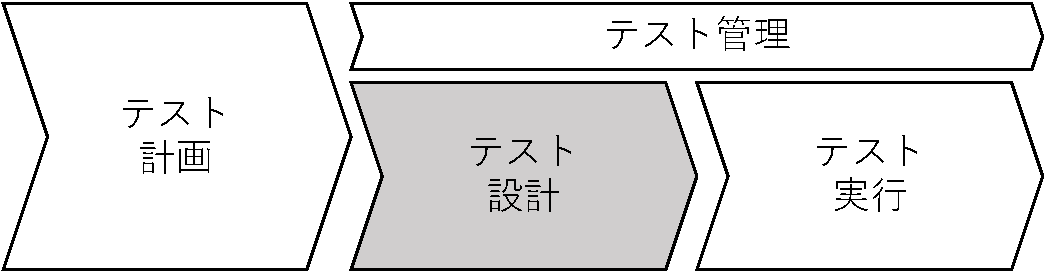
\includegraphics[clip,width=12cm]{test-task.pdf}
    \caption{テストにおけるタスク}
    \label{testtask}
  \end{center}
\end{figure}

\subsubsection{テストの種類}

テスト工程は,表\ref{test-variety}のようにテスト対象の粒度によって単体テスト,結合テスト,システムテストの3種類に分類される.

\begin{table*}[t]
\caption{テストの種類}
\label{test-variety}
\begin{tabular}{|l|p{11cm}|}
\hline
\textbf{テスト粒度}                   & \textbf{説明}                                                                                                       \\ \hline
\textbf{単体テスト}        & プログラムを構成する比較的小さな単位の部品が,個々の機能を正しく果たしているかどうかを検証するテスト \\ \hline
\textbf{結合テスト} & 個々の機能を果たすプログラムの部品(単体)を組み合わせて,仕様通り正しく動作するかを検証するテスト\\ \hline
\textbf{システムテスト}            & 個々の機能や仕組みを総合した全体像のシステムとして,仕様通り正しく動作するかを検証するテスト \\ \hline
\end{tabular}
\end{table*}

単体テストは,クラスやメソッドを対象としたプログラムを検証するためのテストであり,テスト工程の中で最も小さい粒度のテストである.単体テスト設計タスクで作成されるテストケースは,テストプロセス,テスト入力値,テスト期待値から構成される.テストプロセスに従ってテスト対象のソフトウェアにテスト入力値を与え,その出力結果をテスト期待値と比較する.これが一致していればテストは合格となり,一致しなければ不合格となる.単体テスト設計タスクにおいては多くの場合,同値分割法,境界地分析法などのテストケース作成技法を用いてテスト入力値を作成するが,ソフトウェアの要求通りに動作するかを確認するために,多くのバリエーションのテスト入力値を作成する必要がある.

実行した単体テストが十分に行われているかを測定する基準の一つとして,コードカバレッジ(以下,カバレッジ)がある.カバレッジとは,テスト実行時にプロダクションコードが実行された割合を示す.カバレッジは,どのような基準で測定するかによって値が異なる.以下に本研究で扱う代表的な2つのカバレッジの測定方法を説明する.

\begin{description}
\item[命令網羅(C0)]~\\
命令網羅(C0)は,プログラム中に定義されたすべての「命令」について,1回以上実行されたか否かについて判定する測定方法である.Java言語での「命令」は,ソースコードレベルでのステートメントを基準とする方法と,バイトコード上のインストラクション(実行命令)を基準とする方法の2つがある.どちらの場合でも命令網羅率が100\%であることは,単体テストでプログラム内の全命令を少なくとも1回は実行していることを示す.
\item[分岐網羅(C1)]~\\
分岐網羅(C1)は,プログラム中の各分岐について,1回以上実行されたか否かについて判定する測定方法である.Java言語での分岐とはif文やswitch文などの条件分岐,try-catch構文による例外処理などが相当する.分岐網羅率が100\%であることは,単体テストでプログラムのすべての条件分岐が実行されていることを示す.
\end{description}




\subsubsection{テストスメル}

本節では,テストコードの品質を定量的に測定するための基準であるテストスメルについて説明する.

テストスメルとは,テストコードの良くない実装を示す指標である.プロダクションコードの設計だけでなく,テストコードを適切に設計することの重要性は元々Beckら\cite{h1}によって提唱された.さらに,Deursenら\cite{t1}は11種類のテストスメルのカタログ,すなわちテストコードの良くない設計を表す実装とそれらを除去するためのリファクタリング手法を定義した.このカタログはそれ以降,19個の新しいテストスメルを定義したMeszaros\cite{b6}によって拡張された.最近の研究では,これらのテストスメルがソフトウェア開発にもたらす影響について実証的な調査をしている.Bavotaら\cite{Bavota}は,18のソフトウェアプロジェクトにおけるテストスメルの拡散及びソフトウェアの保守に対するテストスメルの影響を調査した.その結果,JUnitクラスの82\%が少なくとも1つのテストスメルの影響を受けていること,さらにテストスメルが存在するクラスは,開発者の理解や不具合特定に悪影響を与えること明らかにした.Tufanoら\cite{Tufano}は,ソフトウェアのライフサイクルにおけるテストスメルの重要性とその寿命を測定することを目的とした実証実験を行った.その結果,開発者はテストクラスに対して最初のコミットでテストスメルを導入し,およそ80\%のケースでテストスメルが除去されないことが分かった.Davideら\cite{Davide}は,テストスメルが存在するテストコードは,そうでないテストコードと比べて変更が多く実施され,テスト対象コードは不具合を含んでいる可能性が高いことを示した.また,テストスメルの存在は開発者のテストコードの理解に悪影響を与えるだけでなく,テストコードがプロダクションコード内の不具合を特定するのにあまり効果的でないと報告した.

以下に,現在提案されているテストスメルの内,本研究で扱う6種類のテストスメルを説明する.

\begin{itemize}
\item Assertion Roulette
\item Default Test
\item Conditional Test Logic
\item Eager Test
\item Exception Handling
\item Mystery Guest
\end{itemize}

以降,それぞれのテストスメルについて説明する.

\begin{description}
\item[Assertion Roulette]~\\
Assertion Rouletteは,図\ref{AR}のようにテストメソッド内に複数のassert文が存在する場合に発生する.各assert文は異なる条件をテストするが,開発者には各assert文のエラーメッセージは提供されない,そのためassert文の1つが失敗した場合,失敗の原因を特定するが困難である.

\begin{figure}[h]
  \begin{center}
    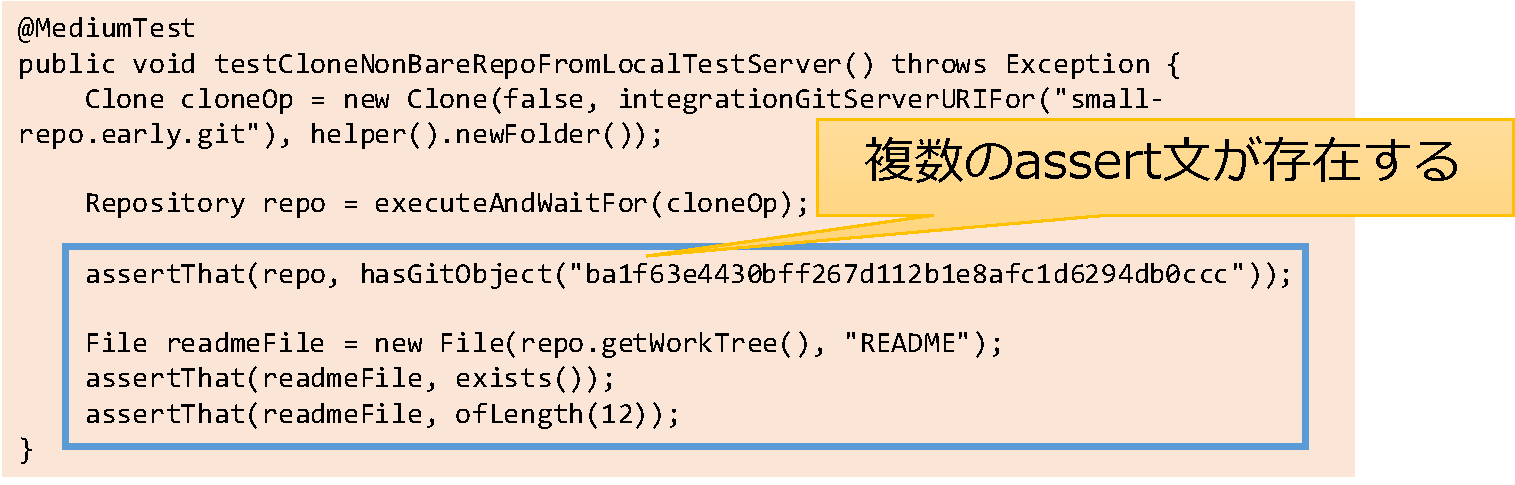
\includegraphics[clip,width=15cm]{AR.pdf}
    \caption{Assertion Rouletteの例}
    \label{AR}
  \end{center}
\end{figure}

\item[Default Test]~\\
Default Testは,図\ref{DT}のようにテストメソッド名が初期状態(意味のない名前)である場合発生する.テスティングフレームを使用した場合,クラス・メソッド名が初期状態である.テストコードの可読性向上のために適切な名前に変更する必要がある.


\begin{figure}[h]
  \begin{center}
    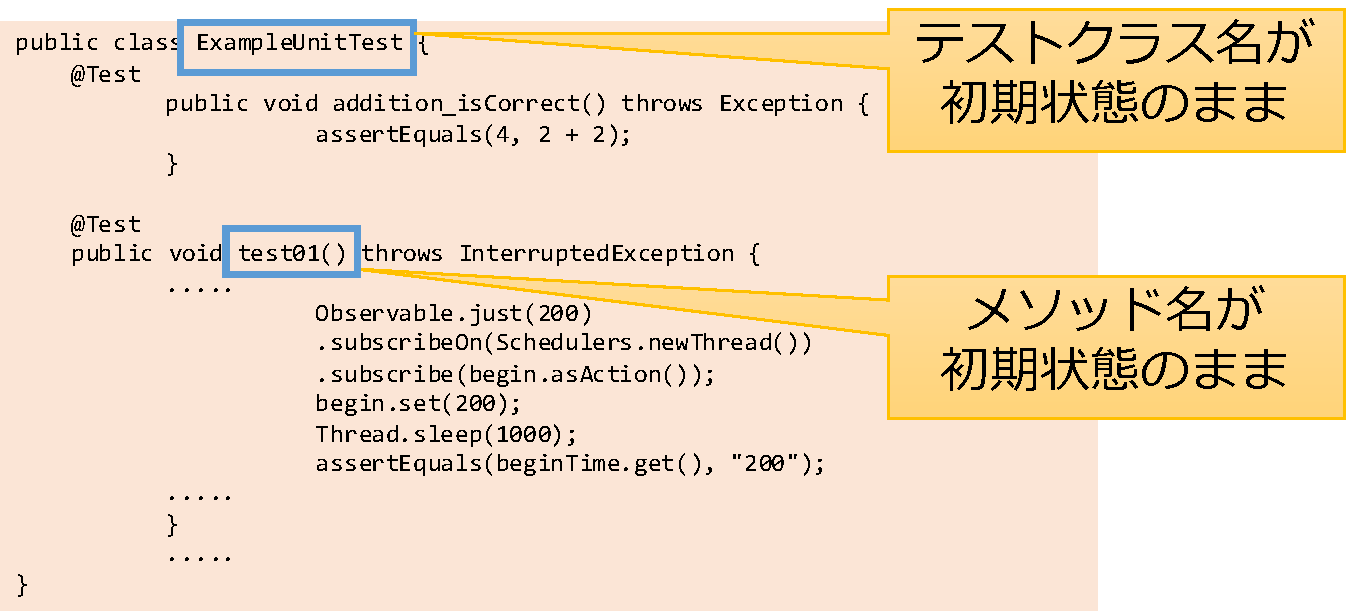
\includegraphics[clip,width=15cm]{DT.pdf}
    \caption{Default Testの例}
    \label{DT}
  \end{center}
\end{figure}

\newpage
\item[Conditional Test Logic]~\\
Conditional Test Logicは,テストメソッド内に複数の制御文が含まれている場合に発生する(図\ref{CTL}).テストの成功・失敗は,制御フロー内にあるassert文に基づくのでテスト結果を予測できない.また,条件分岐が多く複雑なテストコードは可読性を下げる.



\item[Eager Test]~\\
Eager Testは,テストメソッド内でテスト対象クラスのメソッドを複数回呼び出す場合に発生する(図\ref{ET}).1つのテストメソッドで複数のメソッドを呼び出すと,他の開発者は,どのテスト対象をテストするのか混乱が生じる.


\item[Exception Handling]~\\
Exception Handlingは,テストメソッド内に例外処理が含まれている場合に発生する(図\ref{EH}).例外処理は,対象コードに記述すべきで,テストコード内では正しく例外処理が行われるかを確認すべきである.

\item[Mystery Guest]~\\
Mystery Guestは,図\ref{MG}のようにテストメソッド内で外部リソースを利用した場合に発生する.テストメソッド内だけでなく外部ファイルなど,外部リソースを使用すると見えない依存関係が生じる.何らかの影響で外部ファイルを削除されるとテストが失敗してしまう.

\begin{figure}[htbp]
  \begin{center}
    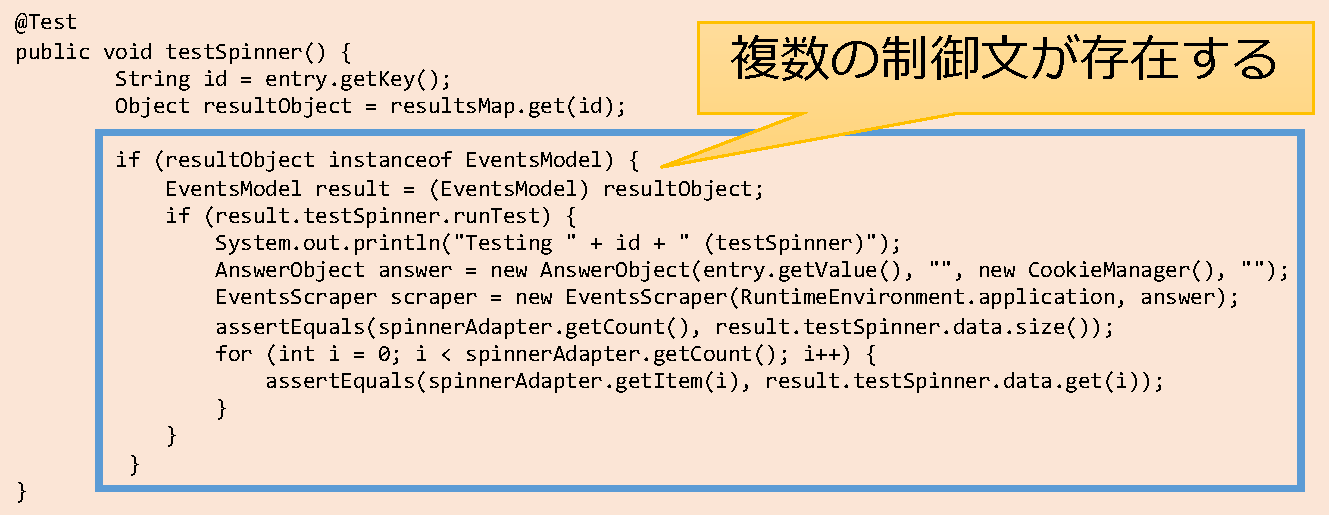
\includegraphics[clip,width=15cm]{CTL.pdf}
    \caption{Conditional Test Logicの例}
    \label{CTL}
  \end{center}
\end{figure}

\begin{figure}[htbp]
  \begin{center}
    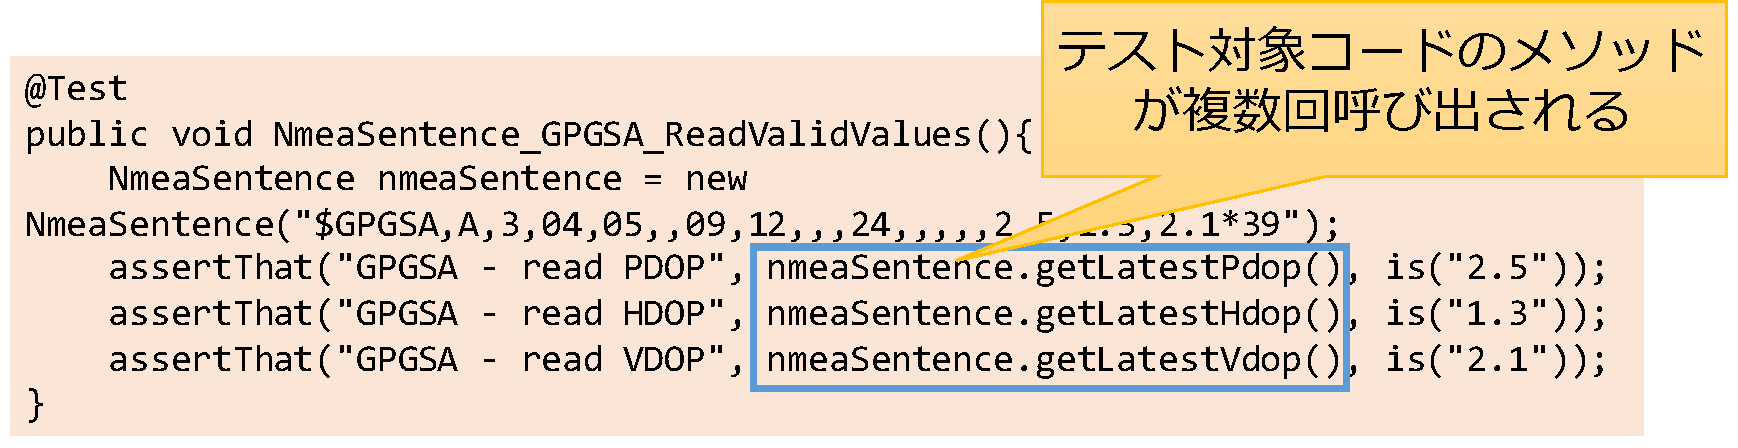
\includegraphics[clip,width=15cm]{ET.pdf}
    \caption{Eager Testの例}
    \label{ET}
  \end{center}
\end{figure}

\begin{figure}[htbp]
  \begin{center}
    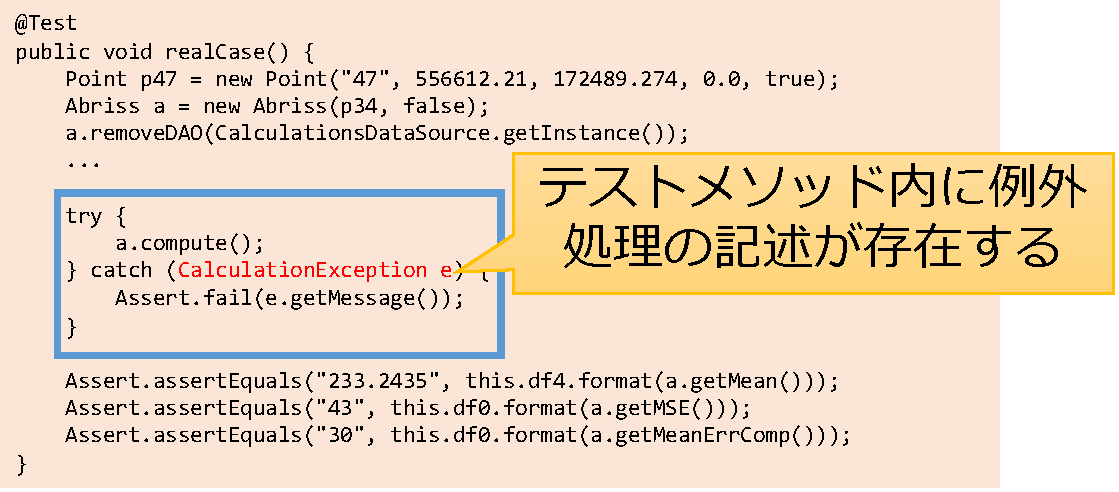
\includegraphics[clip,width=15cm]{EH.pdf}
    \caption{Exception Handlingの例}
    \label{EH}
  \end{center}
\end{figure}

\begin{figure}[htbp]
  \begin{center}
    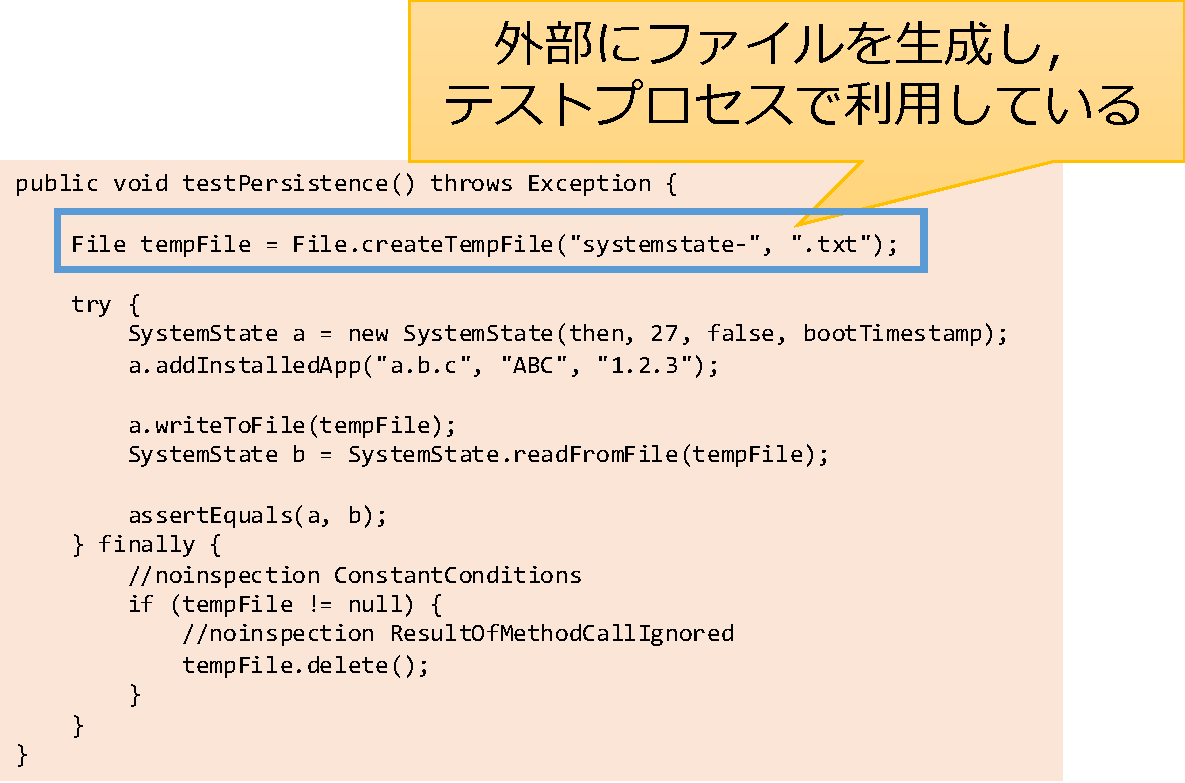
\includegraphics[clip,width=15cm]{MG.pdf}
    \caption{Mystery Guestの例}
    \label{MG}
  \end{center}
\end{figure}
\end{description}


\begin{comment}
\newpage
Bavotaら\cite{Bavota}は,18のソフトウェアプロジェクトにおけるテストスメルの拡散及びソフトウェアの保守に対するテストスメルの影響を調査した.その結果,JUnitクラスの82\%が少なくとも1つのテストスメルの影響を受けていること,さらにテストスメルが存在するクラスは,開発者の理解や不具合特定に悪影響を与えること明らかにした.

Tufanoら\cite{Tufano}は,ソフトウェアのライフサイクルにおけるテストスメルの重要性とその寿命を測定することを目的とした実証実験を行った.その結果,開発者はテストクラスに対して最初のコミットでテストスメルを導入し,およそ80\%のケースでテストスメルが除去されないことが分かった.

Davideら\cite{Davide}は,テストスメルが存在するテストコードは,そうでないテストコードと比べて変更が多く実施され,テスト対象コードは不具合を含んでいる可能性が高いことを示した.また,テストスメルの存在は開発者のテストコードの理解に悪影響を与えるだけでなく,テストコードがプロダクションコード内の不具合を特定するのにあまり効果的でないと報告した.

Palombaら\cite{Fabio2016}は,既存の自動生成ツールによって生成されるテストコードは,プロジェクト内にテストスメルを拡散させることを確認した.生成されたJUnitクラス内83\%が,少なくとも1つのテストスメルの影響を受けることを報告した.また,自動生成されたテストコード内では``Assertion Roulette'',``Eager Test'',``Test Code Duplication''の3つのテストスメルが多く検出される特徴があり,いくつかのテストスメルは同時に存在していることがすることを明らかにした.

自動生成ツールによって大量に生成されるテストコードは,プロジェクト内にテストスメルを拡散させ,開発者の可読性と保守性に大きな影響を与える可能性がある.一般にソフトウェアの保守にかかる継続的なコストは,テストコード作成コストをはるかに上回るため,初めに理解しやすく良質なテストコードを作成する必要がある.
\end{comment}

\newpage
\subsubsection{テストコード自動生成技術}
テスト工程の支援するために様々なテストコード自動生成技術が提案されている.既存の研究\cite{Machado2010}は,既存のテストケースを再利用,自動生成,または再適用することによって,ソフトウェア開発のテスト工程における時間とコストを大幅に節約できることを示している.テスト生成技術は,主にランダムテスト(RT),記号実行(SE),サーチベーステスト(SBST),モデルベース(MBT),組み合わせテストの5つに分類できる.SEはさらに静的記号実行(SSE)と動的記号実行(DSE)に分けられる.

既存研究で提案されている{\sf EvoSuite}\cite{EvoSuite}は,単体テスト自動生成における最先端のツールである.{\sf EvoSuite}は,SBSTを実装したツールであり,2011年に発表されて以来{\sf EvoSuite}をベースとした数多くの研究がなされている.SBSTでは,一般的に以下の手順でテストスイート(テストケースのまとまり)を生成する.

\begin{enumerate}
  \item 達成したい要件に対する達成度合いを定量的に評価できる評価関数を設計
  \item 予め用意したテストスイートをテスト対象に対して実行し,実行したテストスイートの評価関数の値を取得
  \item 取得した評価関数の値が優れているテストスイートを元に,ヒューリスティック探索アルゴリズムによって新規にテストスイートを生成
  \item 3で生成したテストスイートをテスト対象に対して実行し,実行したテストスイートの評価関数の値を取得
  \item 設定した探索打ち切り条件を満たすまで,3,4を繰り返し実行
\end{enumerate}

評価関数の設計方法は,テスト実施の観点によって異なる.例えば,SBSTを用いてコードカバレッジ向上を目指したテストを実施する場合,評価関数は分岐網羅率等が用いられる.

SBSTを用いたテストケース自動生成の例を提示する.図\ref{SBST}において,SBSTを用いて分岐1で「$y > 1$」を満たすようなテスト入力値を生成したい場合,評価関数をプログラムが分岐1に到達したタイミングで評価する.このとき,$x$の値が大きいほど評価関数の値も大きくなり,「$y > 1$」を満たす度合いが大きくなると定量的に評価することができる.まず,$x = -10$として実行すると,評価関数の値は,$E = -10$となる.続いて,仮に$x = -5$として実行すると,評価関数の値は,$E = -5$となる.この場合,後者のテスト入力値の方が「$y > 1$」を達成するためには優れているテスト入力値,つまり$x$の値が大きいテスト入力値をベースに,新しいテスト入力値の生成が行われる.それにより徐々に$x$の値が大きいテスト入力値が生成されていき,最終的に$x = 1$等のテスト入力値が取得できる.

\begin{figure}[htbp]
  \begin{center}
    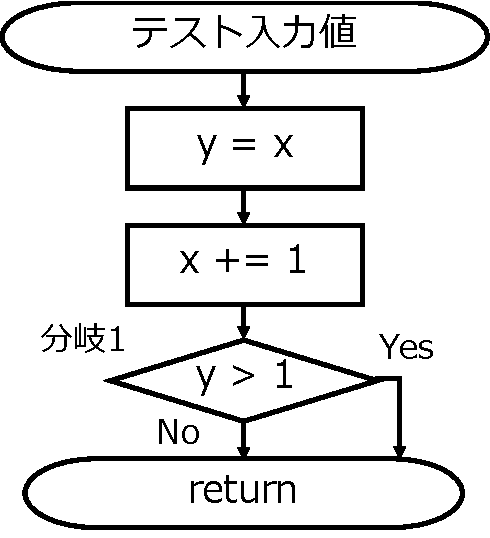
\includegraphics[clip,width=7cm]{SBST.pdf}
    \caption{SBSTによるテストケース生成の例}
    \label{SBST}
  \end{center}
\end{figure}

\subsubsection{既存の自動生成ツールにおける課題}

2.2節では,既存の単体テスト自動生成ツール{\sf EvoSuite}について説明した.単体テストを自動生成することで,開発者は手作業でのテスト作成時間を節約することができ,またコードカバレッジを大幅に向上することができる.しかし,既存ツールによって自動生成されたテストコードは,対象コードの作成経緯や意図に基づいて生成されていないという性質から可読性が低く開発者に信用されていないことや,後の保守作業を困難にするという課題がある\cite{b14,b15,b13}.このことは,自動生成ツールの実用的な利用の価値に疑問を呈する.テストが失敗するたびに,開発者はテスト対象のコード内で不具合の原因を特定するまたは,テスト自体を更新するか否かを判断する必要がある.このようにして,自動生成技術によって一時的に削減できたコストは,後の保守作業を通して返済される可能性がある\cite{b1}.

Palombaら\cite{Fabio2016}は,既存ツールによって自動生成されるテストコードは,プロジェクト内にテストスメルを拡散させることを確認した.自動生成されたJUnitクラス内83\%が,少なくとも1つのテストスメルの影響を受けることを報告した.また,自動生成されたテストコード内では``Assertion Roulette'',``Eager Test'',``Test Code Duplication''の3つのテストスメルが多く検出される特徴があり,いくつかのテストスメルは同時に存在していることがすることを明らかにした.

自動生成ツールによって大量に生成されるテストコードは,プロジェクト内にテストスメルを拡散させ,開発者の可読性と保守性に大きな影響を与える可能性がある.一般にソフトウェアの保守にかかる継続的なコストは,テストコード作成コストをはるかに上回るため,初めに理解しやすく良質なテストコードを作成する必要がある.

我々は,この課題の解決するために既存テストの再利用が有効であると考える.本研究では,OSSに存在する既存の品質の高いテストコード推薦するツールを提案する.既存テストの利用は,コーディング規約や命名規則に従った可読性の高いテストコードを利用できることや,人によって作成された信頼性の高いテストコードを利用できると考える.


\newpage
\section{SuiteRec: テストコード自動推薦ツール}

本章では,本研究で提案するコードクローン検出技術を用いたテストコード自動推薦ツール{\sf SuiteRec}について述べる.本研究では,コードクローン検出技術を利用し,OSS上に存在する既存の高品質なテストコード推薦することで,開発者のテストコード作成を支援することが目的である.{\sf SuiteRec}の基となるアイディアは,クローンペア間でのテストコード再利用である.{\sf SuiteRec}は,開発者からの関数単位の入力コード片に対してその類似コード片を検出する.そして,類似コード片に対応するテストスイートを開発者に推薦する.さらに,推薦されるテストスイート内に含まれるテストスメルを提示し,より品質が高いテストスイートを推薦できるように推薦順位がランキングされる.

図\ref{SO}は,{\sf SuiteRec}によってテストスイートが推薦されるまでの流れを示す.推薦手法は,主に以下の4つのステップから構成される.

\begin{figure}[htbp]
  \begin{center}
    \includegraphics[clip,width=15cm]{pic/SuiteRec-outline.pdf}
    \caption{提案手法の概要}
    \label{SO}
  \end{center}
\end{figure}

\newpage
\begin{description}
\item[Step1]~\\
{\sf SuiteRec}は,開発者から入力コード片を受け取ると,既存のコードクローン検出ツールを用いて,入力コード片に対応する類似コード片を検出する.
\item[Step2]~\\
複数の類似コード片が検出されると,次にその類似コード片に対応するテストスイートをテストコードデータベース内から検索する.
\item[Step3]~\\
各類似コード片のテストスイートが検出されると,次にそれらをテストスメル検出ツールにかけ,各テストスイートに含まれるテストスメルを検出する.
\item[Step4]~\\
最後に,Step1で得られた類似コード片と入力コード片の類似度とStep3で検出されたテストスメルの数を基に出力されるテストスイートの順番がランキングされる.
\end{description}

以降の節で,各ステップの詳細について説明する.

\subsection{Step1: 類似コード片の検出}

Step1では,開発者から受け取った関数単位のコード片に対して類似コード片を検出する.本研究では,コードクローン検出ツールとして{\sf NiCad}\cite{b2}を採用した.{\sf NiCad}は検出対象のコード片のレイアウトを統一的に変換させ,行単位で関数単位のコード片を比較することで,クローンペアを検出するツールであり,このような手法を取ることで,高精度・高再現率でのクローンペアの検出を実現している.

本研究で,{\sf NiCad}を採用した理由として以下の2点が挙げられる.

\begin{itemize}
\item 単体テストの再利用を考える上で関数単位のコード片を高精度で検出できる
\item 構文的に類似したtype2,type3のコードクローンを高速に検出できる
\end{itemize}


{\sf NiCad}は,プロジェクトを入力とし,プロジェクト内のコードクローンをすべて検出する.検出されるコードクローンはクローンクラスとして出力される.{\sf SuiteRec}は,{\sf NiCad}の検出結果の中で入力コード片を含むクローンクラスを特定し,そのクローンクラスに含まれるコード片をすべて類似コード片として扱う.

{\sf SuiteRec}は,{\sf NiCad}を用いて入力コード片に対応する類似コード片を大規模なOSSプロジェクトを保持するGithub\footnote{https://github.com/}のリポジトリから検索する.図\ref{SO}のソースコードデータベースには,テストコードが存在するGithub上の3,205プロジェクトのプロダクションコードが格納されている.具体的には,既存のコード検索エンジンで利用されているデータセット\cite{FaCoY}の内,テストフォルダが存在し,JUnitのテスティングフレームワークを採用しているプロジェクトを選択した.

{\sf NiCad}は,一度に検索できるプロジェクトの規模限度がある.我々は,検索時間を短縮するために検索対象のプロジェクトに前処理をした.具体的には,大規模なプロジェクトは分割し,小規模なプロジェクトは統合させた状態で検索処理を実行した.さらに,検索処理を複数のプロジェクトに対して並列して走らせることで,現実的な時間での類似コードの検索を実現した.また,検出設定については{\sf NiCad}の標準設定で{\sf SuiteRec}に実装した.

\subsection{Step2: テストコードの検索}
Step2では,Step1で検出された類似コード片に対応するテストコードを検索する.大規模なプロジェクトのテストコードが格納されているテストコードデータベース(以下,TDB)からテストコードを検出するために,テスト対象コードとテストコードの対応付けを行う.

本研究では,対象コードとテストコードを対応付けるために以下の3つのフェーズを実施する.

\begin{enumerate}
  \item 命名規則によるクラス単位での対応付け
  \item テストコードを静的解析し,各テストケースから呼び出されるすべてのメソッド名を収集する
  \item テストメソッド名を区切り文字や大文字で分割し,対象メソッドと部分一致した場合,テストコードと対象コードをメソッド単位で対応付ける
\end{enumerate}

本研究では,テストコードとしてJUnitテスティングフレームワークを用いた単体テストを対象とする.フェーズ1では,JUnitの命名規則に従ってテストクラス名の先頭または,末尾に``Test''という文字列が含まれるテストクラスを収集し,収集したテストクラスから``Test''を除いたクラス名をテスト対象クラスとする.例えば,CalculatorクラスとCalculatorTestクラスが対応付けられる.

フェーズ2では,テストコードを静的解析し,テストメソッド内で呼び出されるメソッド名を取得する.単体テストでは,図\ref{map}の例のようにテストコード内でオブジェクトの生成を行い,テスト対象コードのメソッド呼び出して実行される.すなわち,TCD内のテストコードを静的解析し,メソッド呼び出しを取得することで,テスト対象コードとテストコードを対応付ける.ただし,テストメソッド内では,複数のメソッドが呼び出されていることも考えられるので,フェーズ3では,さらにメソッド名の比較も行う.テストメソッド名の記述方法としてテスト対象メソッドの処理の内容を忠実に表すことが推奨されており,対象メソッドの名前が記述されていることが多い\cite{b22}.従って,テストメソッドの名前を区切り文字や大文字で分割し,対象メソッドと部分一致した場合,対応付けるように実装した.

\begin{figure}[htbp]
  \begin{center}
    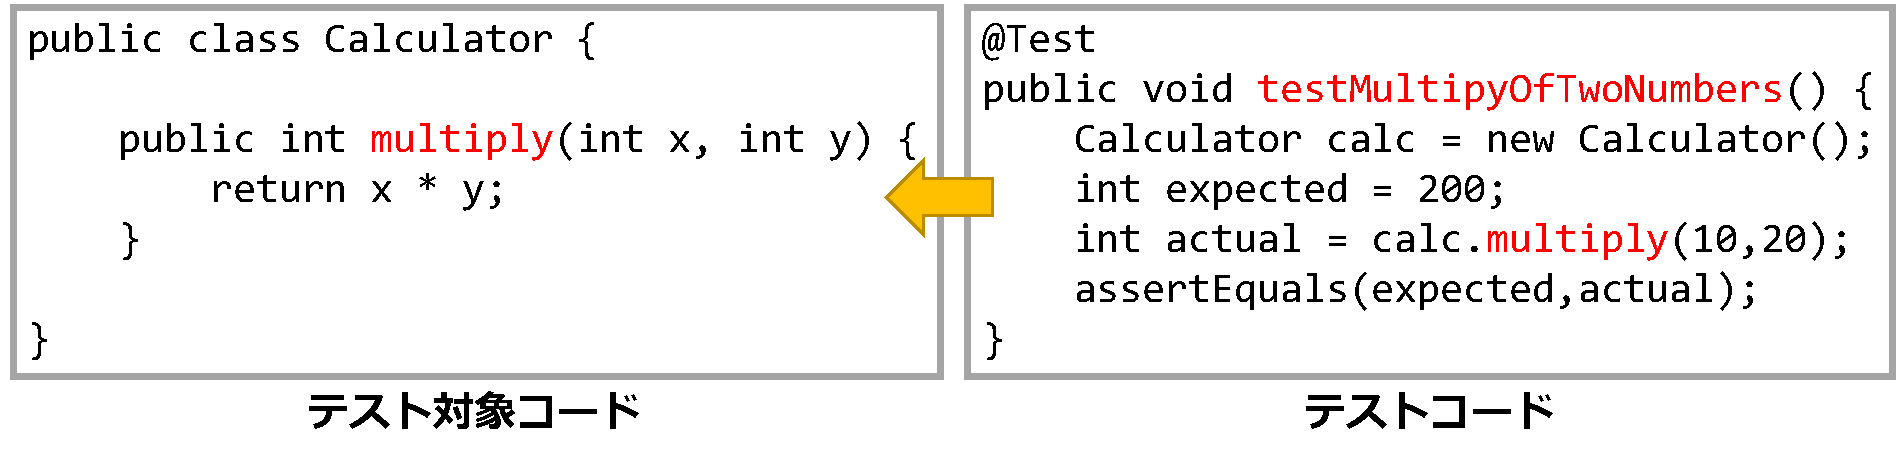
\includegraphics[clip,width=15cm]{pic/mapping.pdf}
    \caption{テストコードと対象コードの対応付け}
    \label{map}
  \end{center}
\end{figure}

\subsection{Step3: テストスメルの検出}

Step3では,Step2で検索されたテストスイート内のテストスメルを検出する.本研究では,テストスメル検出ツールとして{\sf tsDetect}\footnote{https://testsmells.github.io/}\cite{Peruma}を採用した.{\sf tsDetect}はASTベースの検出手法で実装されたツールであり,19種類のテストスメルを検出できるツールである.また,85\%〜100\%の精度と90\%〜100\%の再現率でテストスメルを検出できる.{\sf tsDetect}は,既存研究で利用実績があり高精度で多くのテストスメルを検出できるので本研究でも利用した.本研究では,{\sf tsDetect}で検出できる19種類のテストスメルの内,2.2.2節で説明したテストコードの推薦を考える上で重要な6種類のテストスメルを提示するように実装した.

{\sf tsDetect}は,ASTベースの検出手法であり大規模なテストコードに対して実行すると計算コストが高い.我々は,事前にTDB内のテストコードのテストスメルを検出しその情報をテストコードに対応付けてTDBに格納した.これにより,推薦プロセスにおけるテストスメル検出時間を短縮化した.また,推薦テストコードとして相応しくない以下の4つのテストスメルを含むテストコードを事前にTDBから除去し,推薦されるテストコードとして出力されないようにした.

\begin{itemize}
\item \textbf{Empty Test} : テストメソッド内にテストの記述が無く,コメントのみが含まれているテストコード
\item \textbf{Ignored Test} : @Ignoreアノテーションがあり,実行されないテストコード
\item \textbf{Redundant Assertion} : 必ずテストが成功する意味のないテストコード
\item \textbf{Unknow Test} : assert文が存在しないテストコード
\end{itemize}

\subsection{Step4: 推薦されるテストスイートの順位付け}

最後のStep4では,推薦されるテストスイートを順位付けし,開発者が参考にしたいテストスイートを上位に提示できるようにテストスイートの並び替えを行う.

{\sf SuiteRec}の順位付けは,Step1の入力コード片と類似コード片の類似度とStep3で検出されたテストスメルの数を基に計算する.我々は,以前の調査\cite{fose2019}で,クローンペア間とテストコードの類似度の関係を調査した.詳細には,OSS上に存在する3つの有名Javaプロジェクト内にある両方のコード片にテストコードが存在するコードクローンを対象に,クローンペア間の類似度とそれぞれのコード片に対応するテストコードの類似度の関係を調査した.その結果,テストコード間の類似度と対象のクローンペア間の類似度には相関関係があり,クローンペア間の類似度が高いほどテストコードを再利用できる可能性が高いことが分かった.{\sf SuiteRec}では,この結果を基に類似度が高いクローンペアの順に並び替え,さらに類似度が同じ場合,テストスメルの数で推薦するテストスイート順位を決定するように推薦ランキングを実装した.

本研究では,クローンペア間の類似度を{\sf NiCad}で用いられる計算方法である{\it Unique Percentage of Items} (以下,{\it UPI} )を利用して計算する.以下に,{\it UPI}の計算式を示す.

\[
  Unique\, Percentage\, of\, Items\, (UPI) =
  \frac{No.\, of\, Unique\, Items * 100}{Total\, No.\, of\, Items}
\]

\vspace{\baselineskip}

ここで,{\it No.of Unique Items}は,入力コード片と類似コード片を行単位で比較した際に一致した行の数を意味する.{\it Total No.of Items}は,コード片内のすべての行の数を意味する.比較対象のコード片の{\it Total No.of Items}が異なる場合,行数が大きい方の{\it Total No.of Items}を用いて計算する.例えば,入力コード片の行数が10,類似コード片の行数が12で,一致した行数が9の場合,入力コード片と類似コード片の類似度は75\%になる.

\begin{figure}[htbp]
  \begin{center}
    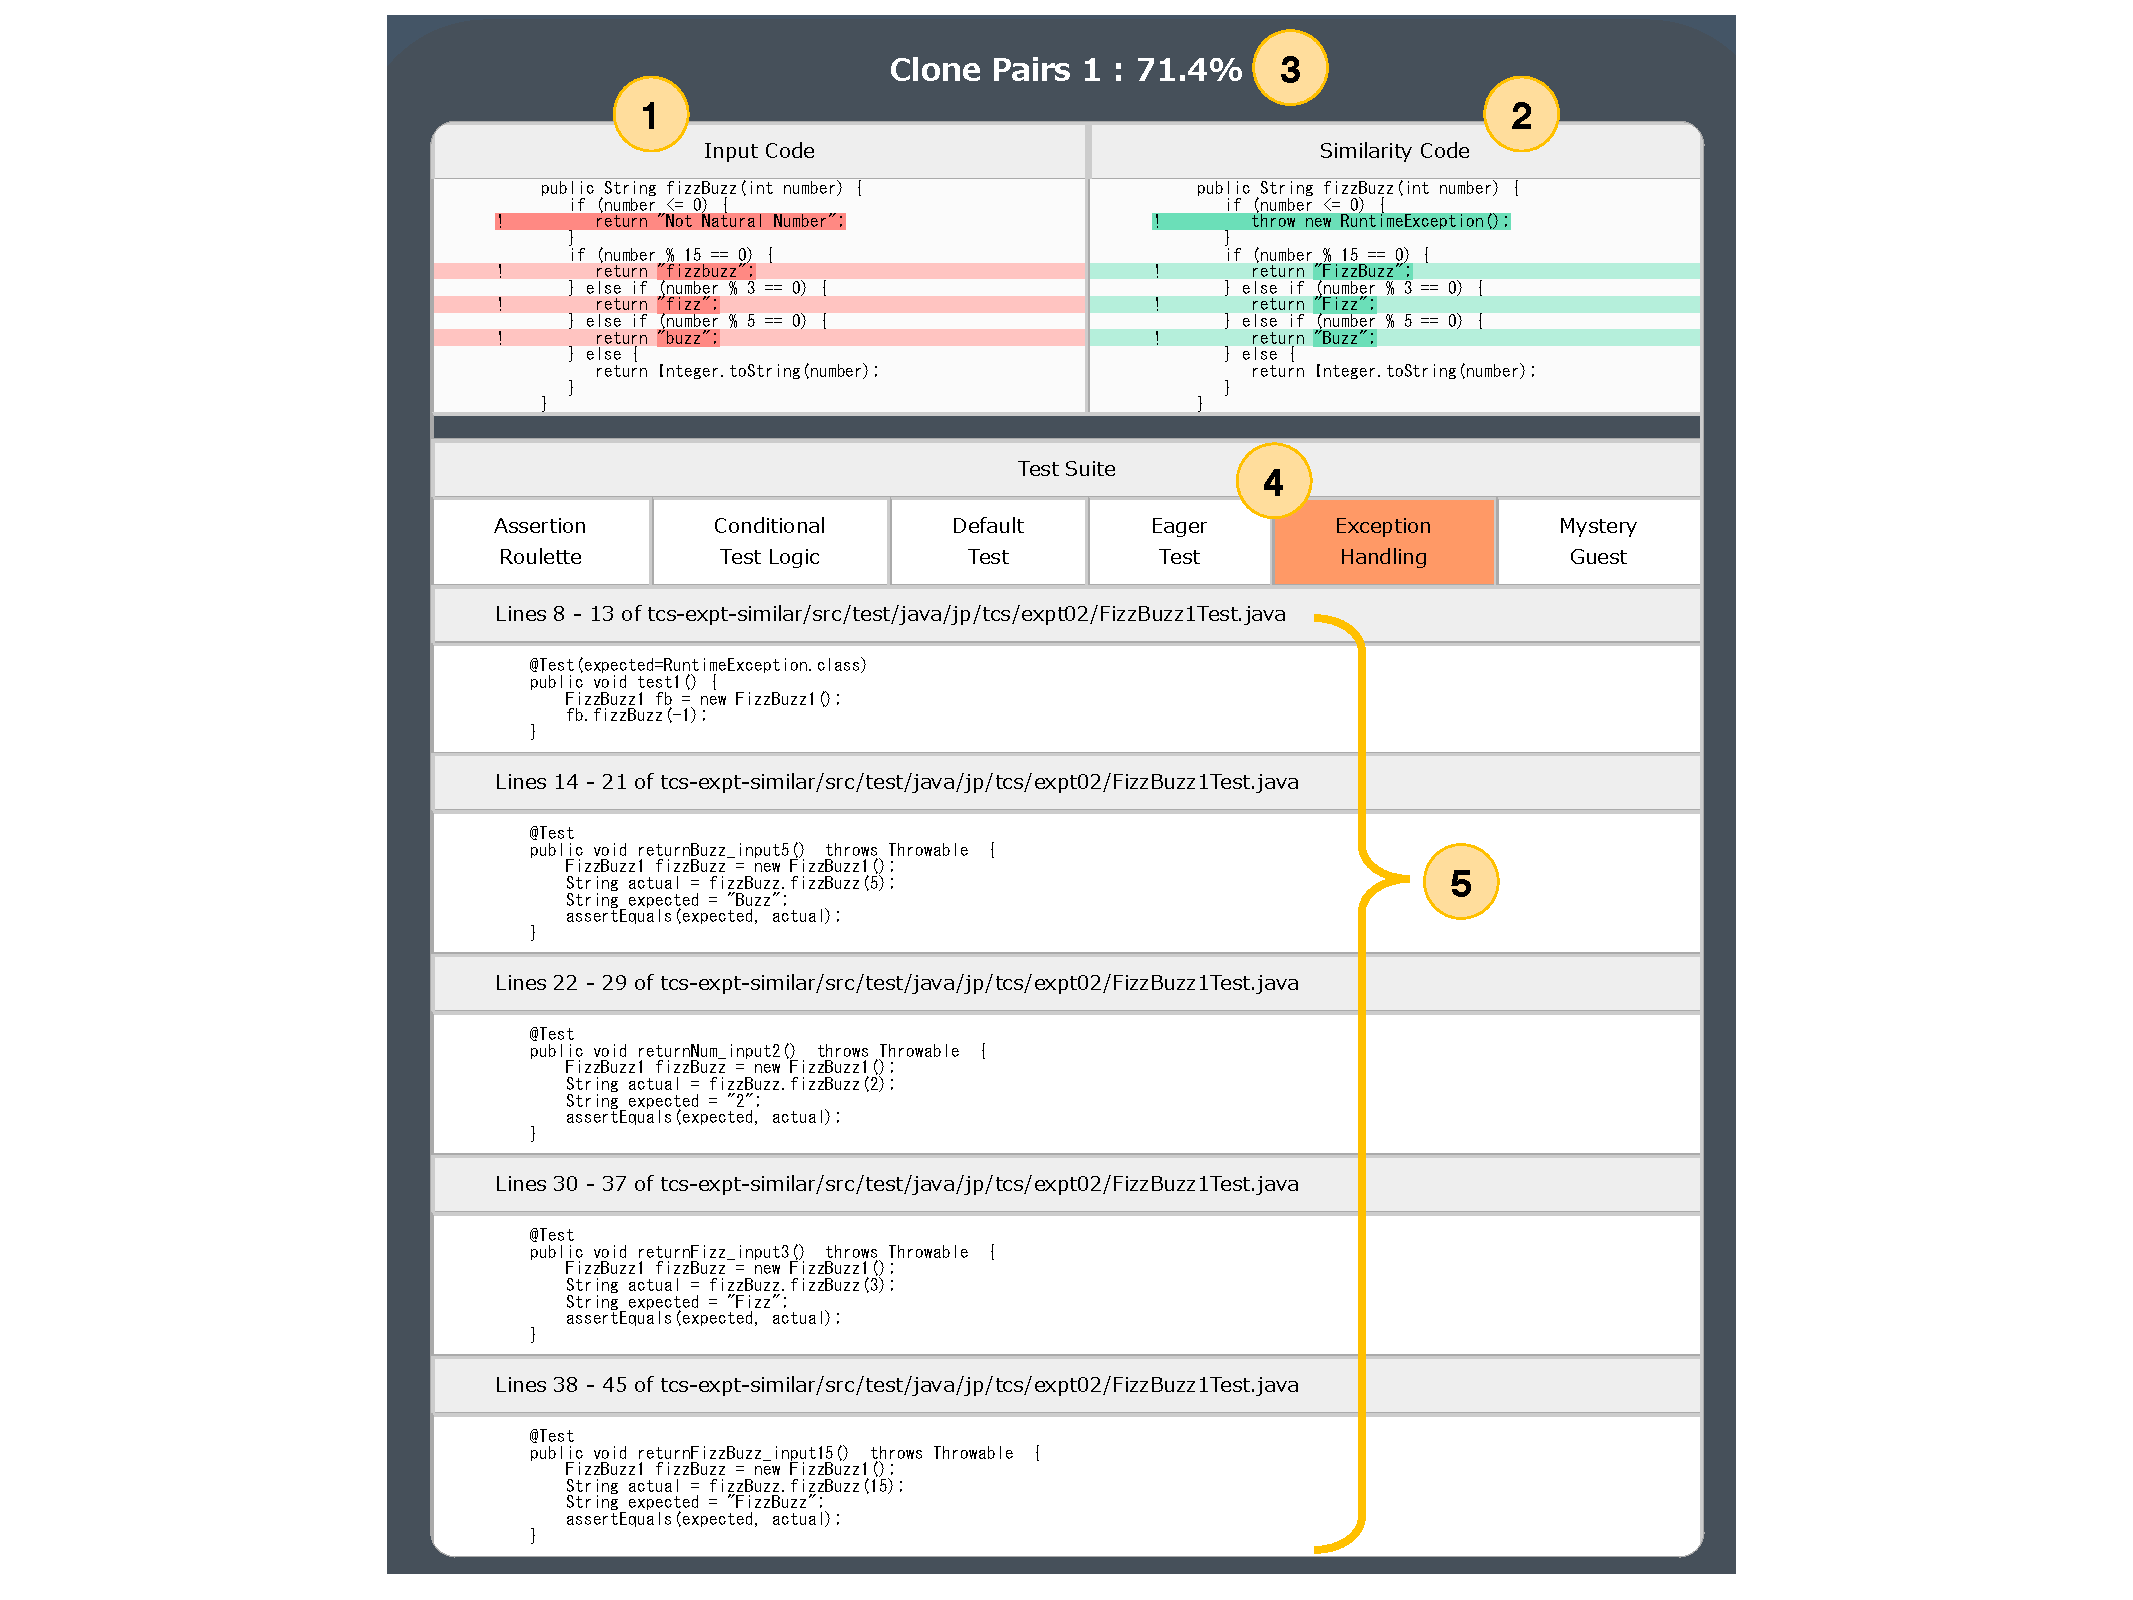
\includegraphics[clip,width=15cm]{SuiteRec.pdf}
    \caption{{\sf SuiteRec}から推薦されるテストコード}
    \label{SR}
  \end{center}
\end{figure}

\newpage
図\ref{SR}は{\sf SuiteRec}から推薦されるテストコードの例である.以下に{\sf SuiteRec}のインターフェースについて各項目の説明を示す.


\begin{enumerate}
\renewcommand{\labelenumi}{(\arabic{enumi})}
\item{\textbf{Input Code Fragment.}開発者が入力した関数単位のプロダクションコードが表示される.}
\item{\textbf{Similarity Code Fragment.}入力コードに対する類似コードが表示される.入力コードと類似度コードの違いが分かるように差分がハイライトされる.}
\item{\textbf{Degree of similarity.}入力コードと類似コードの類似度が表示される.類似度はNICADで用いられている計算方法Unique Percentage of Items (UPI)を採用した.}
\item{\textbf{Test Smells.}推薦されるテストスイート内にテストスメルが含まれている場合,そのテストスメルがオレンジ色にハイライトされ開発者にテストスメルの存在を提示する.}
\item{\textbf{Recommend Test Suites.}推薦されるテストスイートが表示される.また,どのプロジェクトからテストコードが参照されたのかを示すためにファイルパスも表示される.}
\end{enumerate}

\newpage
\section{評価実験}

この章では,{\sf SuiteRec}を定量的及び定性的に評価するために,被験者による評価実験について説明する.評価実験は,主に以下の2つの実験を実施した.

\begin{itemize}
\item \textbf{評価実験1} : テストコード作成支援に関する実験
\item \textbf{評価実験2} : 推薦テストコードの順位付けに関する実験
\end{itemize}

以降,各評価実験の詳細について説明する.

\subsection{評価実験1: テストコード作成支援に関する実験}
評価実験1では,{\sf SuiteRec}が開発者のテストコードをどの程度支援できるかを評価する.被験者に3つのプロダクションコードのテストコードを作成してもらい,{\sf SuiteRec}を使用して作成した場合とそうでない場合のテストコードを比較することで評価を行う.実験を通してコードカバレッジ,実験タスクを終了するまでの時間及びテストコードの品質に関するデータを収集することで,以下のリサーチクエスチョンに答えることを目指す.

\begin{description}
\item[\textbf{RQ1: {\sf SuiteRec}は高いカバレッジを持つテストコードの作成を支援できるか?}]~\\
RQ1では,被験者が作成したテストコードのカバレッジを測定する.テスト工程において,ソフトウェアの品質を確認する1つの指標としてカバレッジは重要な要素である.テストコード内で一度も実行されない行が存在するとその部分の品質を確保することはできない.{\sf SuiteRec}の利用は高いカバレッジを達成するために役に立つのか?
\item[\textbf{RQ2: {\sf SuiteRec}はテストコードの作成時間を削減できるか?}]~\\
RQ2では,被験者のテストコード作成タスクに費やす時間を測定する.開発者は{\sf SuiteRec}で推薦されるテストコードを参考にすることで,テストコード作成時間を短縮化できるのか?
\item[\textbf{RQ3: {\sf SuiteRec}はテストスメルの数が少ないテストコードの作成を支援できるか?}]
RQ3では,被験者が作成したテストコード内に含まれるテストスメルを検出し,テストコードの品質を測定する.開発者は{\sf SuiteRec}で推薦されるテストコードを参考にすることで,品質の高いテストコードを作成することができるのか?
\item[\textbf{RQ4: {\sf SuiteRec}の利用は,開発者のテストコード作成タスクの認識にどう影響するか?}]
RQ4では,テストコード作成タスクを完了した被験者に作成タスクに関するアンケート回答してもらった.{\sf SuiteRec}を利用した場合,テストコードの作成が容易になり,自身で作成したテストコードに自信が持てるのか?
\end{description}
%\item[\textbf{RQ5: {\sf SuiteRec}は,開発者が求める順番でテストスイートをランキングできるか?}]~\\
%RQ5では,SuiteRecから推薦されるテストスイートのランキングの妥当性を検証する.

以降,4.1.1節では,評価実験1で用いた実験用データセットについて説明する.4.1.2節では,評価実験1の手順について説明する.最後に4.1.3節で,評価実験1の結果について説明する.


\subsubsection{評価実験1のデータセット}

評価実験1を実施するために,基本的なプログラミングスキルを保有し,ソフトウェアテストに関する知識を持つ学生を募集した.そして,情報科学を専攻するの修士過程の学生10人対して実験を実施した.事前アンケートによると9割の学生が2年以上のプログラミング経験があり,8割の被験者が1年以上のJava言語の経験があった.また,すべての学生が授業などの講義でソフトウェアテストに関する基本的な知識を持っており,8割が単体テストの作成経験があった.

評価実験1では,被験者に3つの実験タスクを割り当てた.以降,これら実験タスクをそれぞれ,タスク1,タスク2,タスク3と呼ぶ.被験者はテストコードを作成するのでプロダクションコードの仕様を十分理解していることが前提になる.そこで,我々はプロダクションコードとして競技プログラミングをよく用いられる典型的な計算問題を実験タスクとして選択した.また,各タスクの仕様を確認できるように自然言語で記述された仕様書を用意した.3つの各タスクで違いを出すためにタスク1,2,3の順に条件分岐の数を8,16,24と多くなるように設定した.以下に,各タスクの概要を示す.

\begin{description}
\item[タスク1]~\\
タスク1は,典型的なFizzBuzzのJavaメソッドに対するテストコードを作成するタスクである.このタスクは,被験者が一番始めに実施するタスクであり,条件分岐の数が8で3つのタスクの中で最も単純な構造のプログラムである.以下に,タスク1のプロダクションコードの仕様とソースコードを示す.

\begin{itembox}[l]{タスク1のプロダクションコードの仕様}
整数を入力し,次の条件で結果を返すプログラム.
\begin{itemize}
\item 3で割り切れる場合,``fizz''を返す.
\item 5で割り切れる場合,``buzz''を返す.
\item 3と5両方で割り切れる場合,``fizzbuzz''を返す.
\item 入力が自然数でない場合,``Not Natural Number''を返す.
\item 上記以外は,入力数値をString型で返す.
\end{itemize}
\end{itembox}

\begin{figure}[htbp]
  \begin{center}
    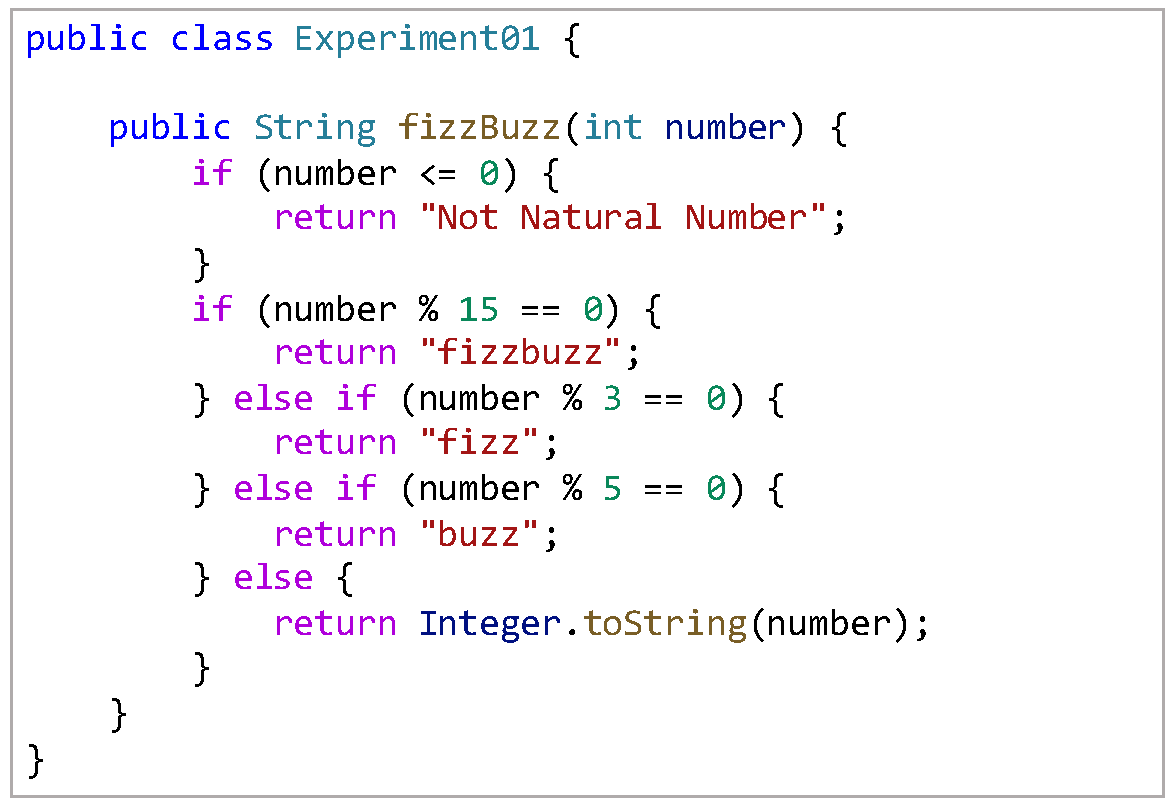
\includegraphics[clip,width=10cm]{E1.pdf}
    \caption{タスク1のプロダクションコード}
    \label{E1}
  \end{center}
\end{figure}

\item[タスク2]~\\
タスク2は,第1引数に応じて残り3つの引数の計算方法を変更し,結果を出力するJavaメソッドのテストコードを作成するタスクである.このタスクは,条件分岐の数が16でタスク1より比較的複雑な構造のプログラムである.以下に,タスク2のプロダクションコードの仕様とソースコードを示す.

\begin{itembox}[l]{タスク2のプロダクションコードの仕様}
第1引数に応じて残り3つの引数の計算方法を変更し,結果を返す.
\begin{itemize}
\item 第1引数が``Medium''の場合,残り3引数の中央値を返す.
\item 第1引数が``max''の場合,残り3引数の最大値を返す.
\item 第1引数が``min''の場合,残り3引数の最小値を返す.
\item 第1引数が上記以外の場合,$-1$を返す.
\end{itemize}
\end{itembox}

\begin{figure}[htbp]
  \begin{center}
    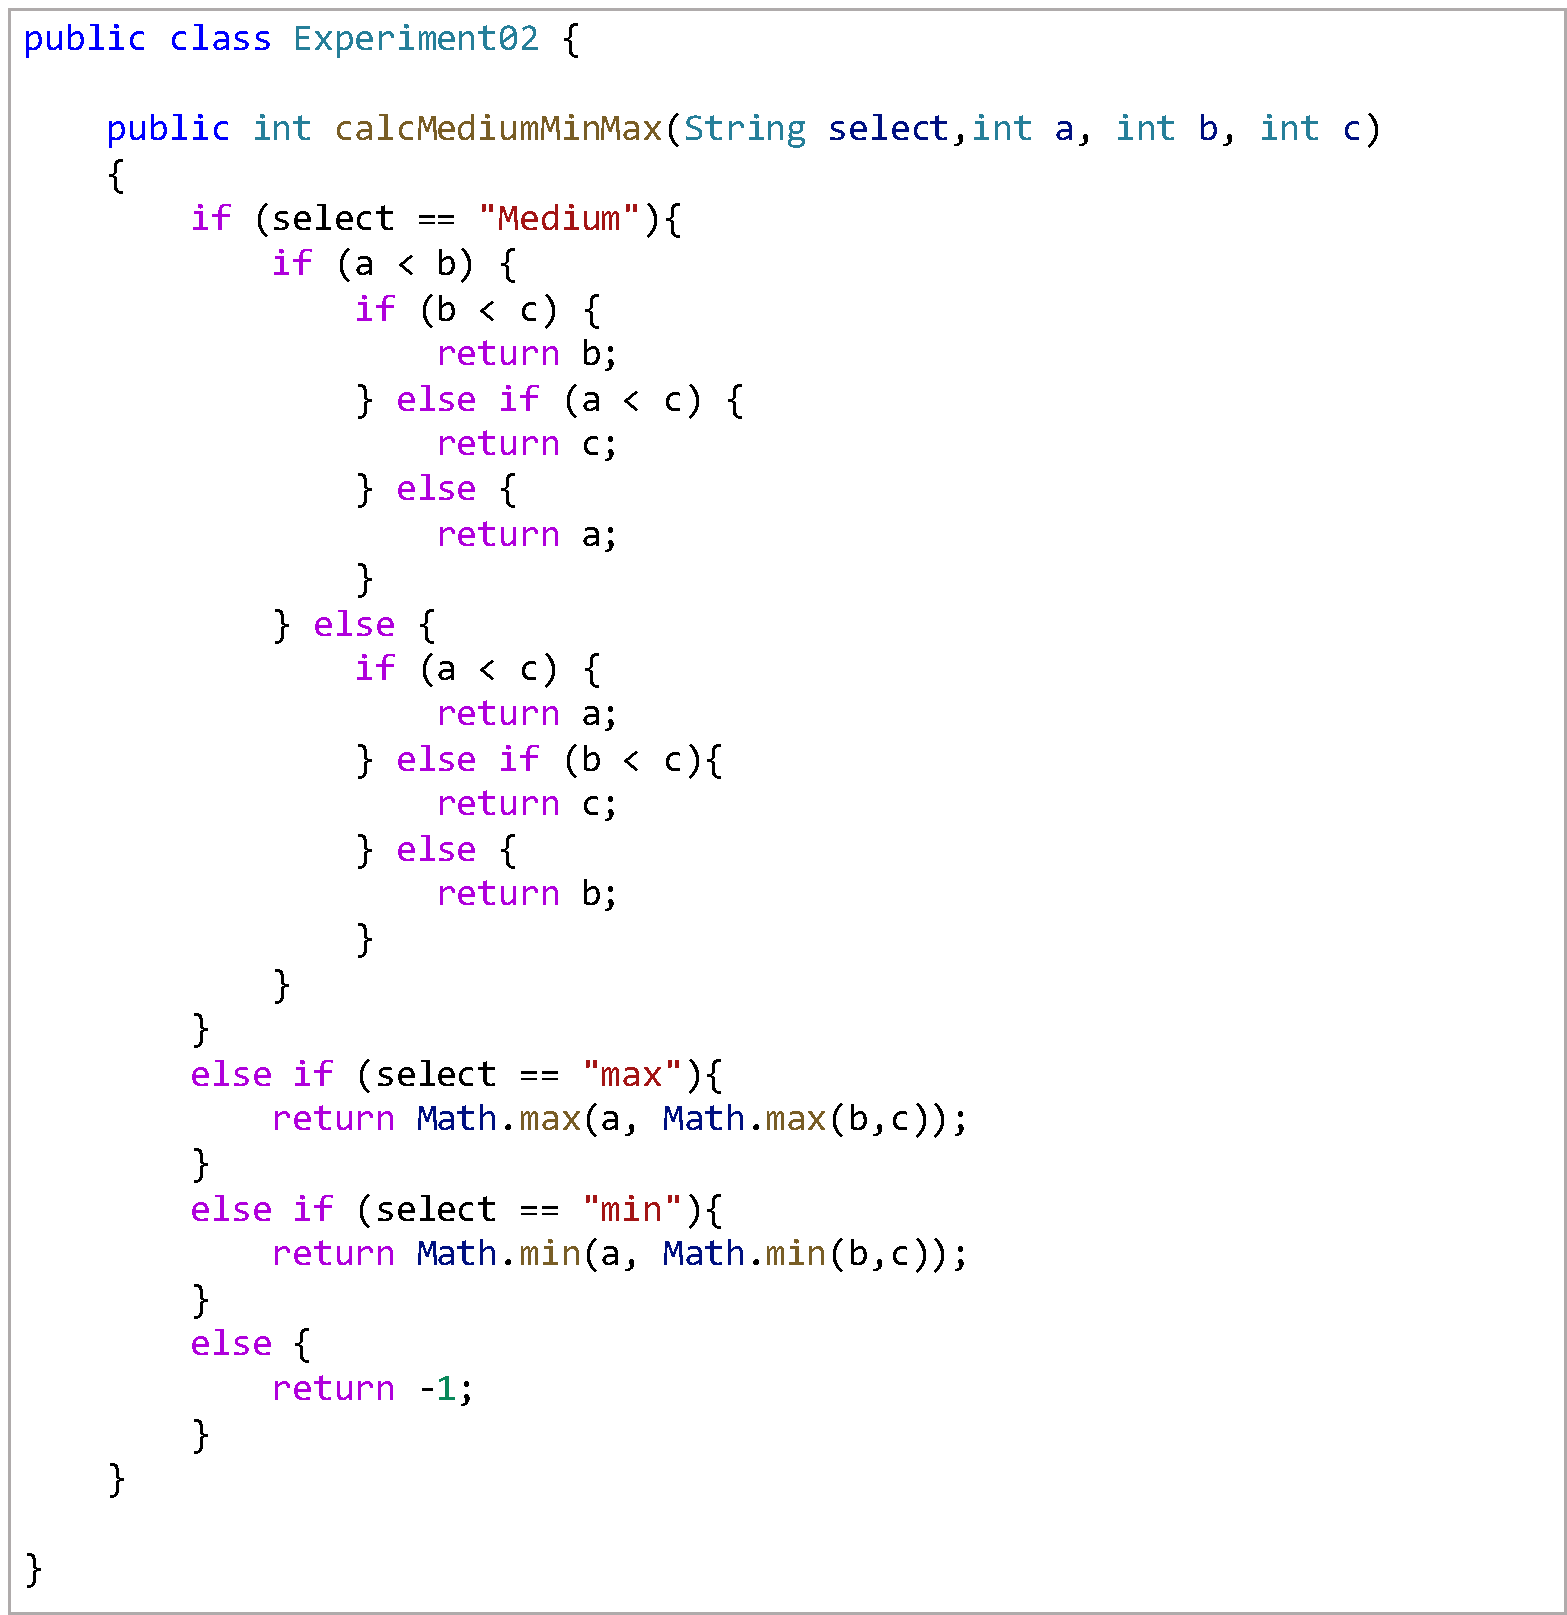
\includegraphics[clip,width=13cm]{E2.pdf}
    \caption{タスク2のプロダクションコード}
    \label{E2}
  \end{center}
\end{figure}


\item[タスク3]~\\
タスク3は,2つのint型の値を入力し,試験の合否を判定するプログラムのテストコードを作成するタスクである.このタスクは,条件分岐の数が24個存在し,3つのタスクの中で最も複雑な構造のプログラムである.以下に,タスク3のプロダクションコードの仕様とソースコードを示す.

\begin{itembox}[l]{タスク3のプロダクションコードの仕様}
2つのスコア(0~100点)を入力し,次の条件に従って合格・不合格を判定するプログラム.
\begin{itemize}
\item スコアが0~100点以外の場合``Invalid Input''を返す.
\item どちらかのスコアが0点であれば``failure''を返す.
\item 両方とも60点以上の場合``pass''を返す.
\item 合計が130点以上の場合``pass''を返す.
\item 合計が100点以上で,どちらかのスコアが90点以上であれば``pass''を返す.
\item 上記以外は``failure''を返す.
\end{itemize}
\end{itembox}


\begin{figure}[htbp]
  \begin{center}
    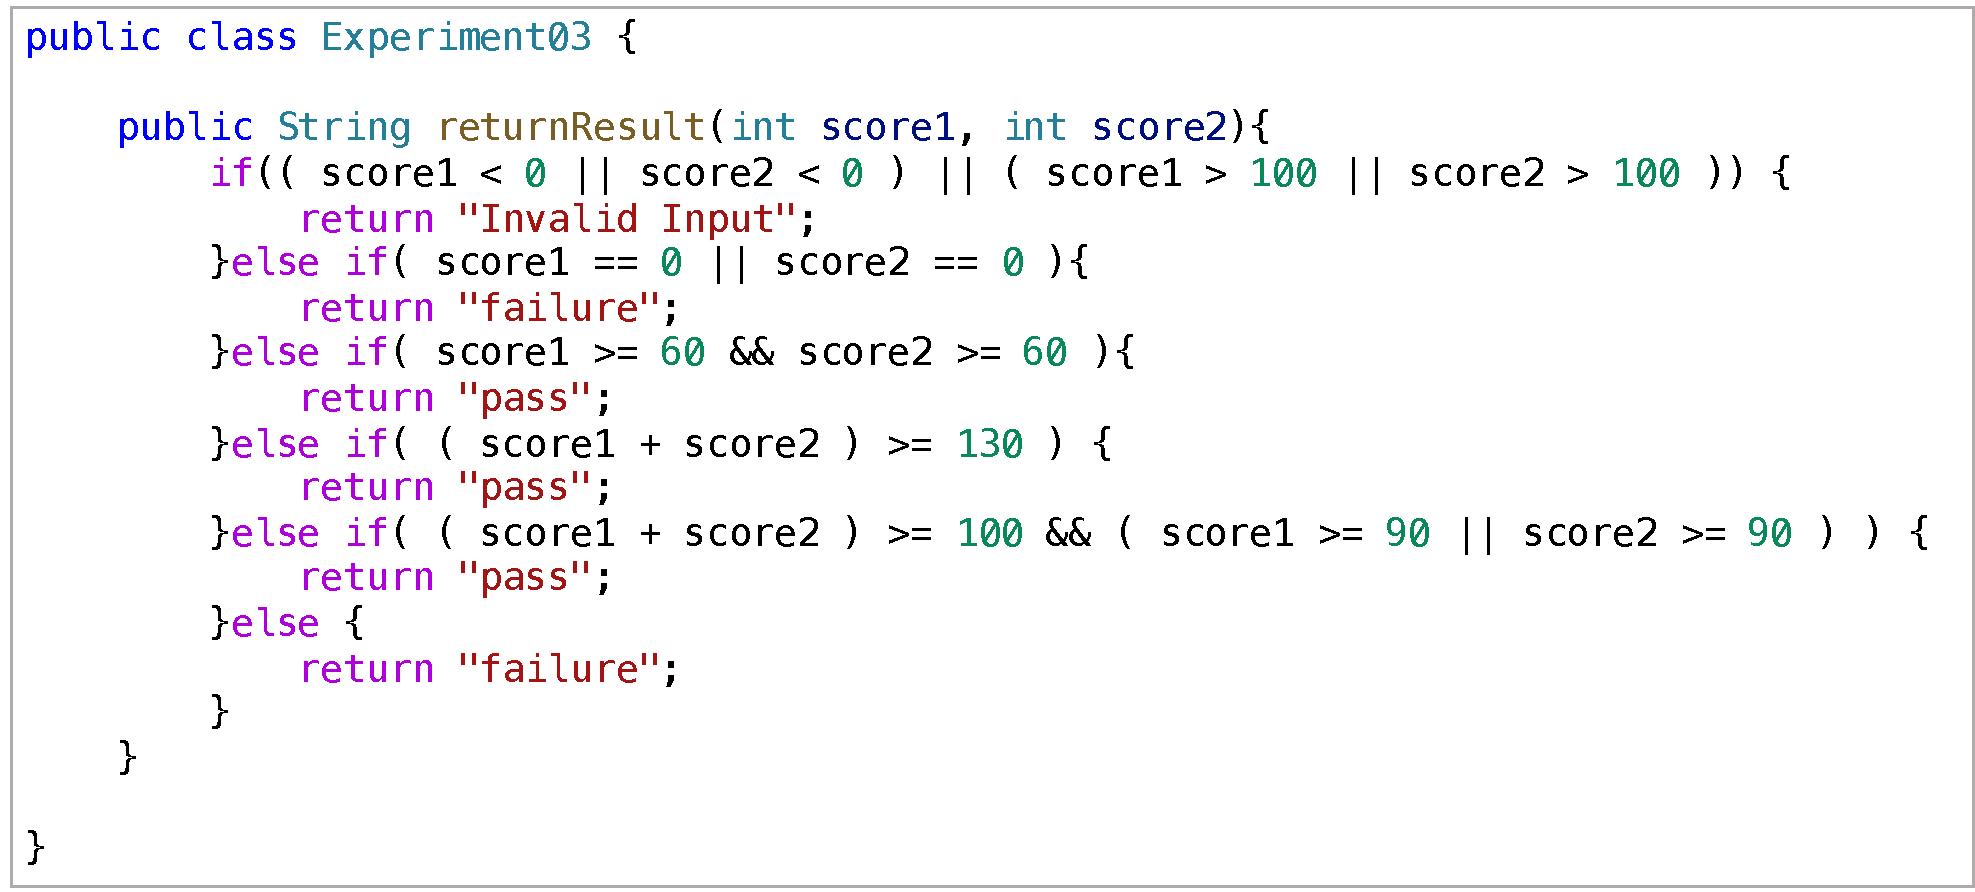
\includegraphics[clip,width=15cm]{E3.pdf}
    \caption{タスク3のプロダクションコード}
    \label{E3}
  \end{center}
\end{figure}

\end{description}

\subsubsection{評価実験1の手順}

4.1節で説明した実験タスクを用いた評価実験1の手順について説明する.まず,被験者間の事前知識の違いによる結果の相違を無くすために,実験前にソフトウェアテストに関する基本的な知識からJUnitの使用に関する30分の講義を実施した.また,被験者に{\sf SuiteRec}の使い方を説明し,実際に練習問題で使用してもらいツールの利用とテストコードの作成について理解していることを確認した.

その後,用意した3つの実験タスクに対してテストコードを作成してもらった.被験者には,与えられた3つタスクを{\sf SuiteRec}を使用した場合とそうでない場合でテストコードを作成してもらった.本実験では,タスクの終了は被験者に判断してもらう.具体的には,被験者自身が作成したテストコードのカバレッジ・品質に満足したとき,実験タスクを終了してもらった.実験時間は1つのタスクにつき最大25分の時間を設けた.我々は,{\sf SuiteRec}の利用効果がタスクによって偏らないように,図\ref{assign}のように被験者を2つのグループに分け,グループによって{\sf SuiteRec}の利用の有無をタスクによって変えるように割り当てた.また,{\sf SuiteRec}を利用した場合の学習効果を防ぐために,3つのタスクで連続して{\sf SuiteRec}を利用しないようにタスクの割り当てを行った.さらに実験中,被験者は過去の回答を参考できないようにした.

\begin{table}[h]
\caption{タスクの割り当て}
\label{assign}
\begin{center}
\begin{tabular}{|c|l|l|l|c|}
\hline
グループ & \multicolumn{2}{c|}{A}                              & \multicolumn{2}{c|}{B}                           \\ \hline
     & \multicolumn{1}{c|}{タスク} & \multicolumn{1}{c|}{ツール} & \multicolumn{1}{c|}{タスク} & ツール                   \\ \hline
1回目  & タスク1                     &                          & タスク1                     & 〇                     \\ \hline
2回目  & タスク2                     & \multicolumn{1}{c|}{〇}   & タスク2                     & \multicolumn{1}{l|}{} \\ \hline
3回目  & タスク3                     &                          & タスク3                     & 〇                     \\ \hline
\end{tabular}
\end{center}
\end{table}


最後に,実験タスク終了後に被験者にテストコード作成に関するアンケートに答えてもらった.以下に,実施したアンケートの項目を示す.被験者は,これらのアンケート項目に対して5段階評価(強く反対・反対・どちらでもない・賛成・強く賛成)で回答してもらった.


\begin{itembox}[l]{評価実験1: 実験タスクに関するアンケート項目}
\begin{description}
\item[Q1.]今回の実験内容(課題)を理解できました.
\item[Q2.]実験タスクを終えるのに十分な時間がありました.
\item[Q3--a.]テストコードの作成は簡単でした(ツール使用).
\item[Q3--b.]テストコードの作成は簡単でした(ツール不使用).
\item[Q4--a.]作成したテストコードのカバレッジに自信がある(ツール使用).
\item[Q4--b.]作成したテストコードのカバレッジに自信がある(ツール不使用).
\item[Q5--a.]作成したテストコードの品質に自信がある(ツール使用).
\item[Q5--b.]作成したテストコードの品質に自信がある(ツール不使用).
\item[Q6.]推薦ツールの使用はテストコードを作成する際に参考になりました.
\end{description}

\end{itembox}

\newpage
\subsubsection{評価実験1の結果}
本節では,評価実験1の被験者による{\sf SuiteRec}の定量的および定性的評価の結果を報告する.本章の前半で説明した,4つのリサーチクエスチョンについての分析結果を提示する.

\paragraph{RQ1: {\sf SuiteRec}は高いカバレッジを持つテストコードの作成を支援できるか?}RQ1では,{\sf SuiteRec}を使用した場合とそうでない場合の被験者が,作成したテストコードのカバレッジを比較する.本実験では,被験者によって提出されたテストコードの命令網羅と分岐網羅の2種類のカバレッジを計算した.カバレッジの計算には,統合開発環境Eclipse\footnote{https://www.eclipse.org/}のプラグインとして搭載されているEclEmma\footnote{https://www.eclemma.org/}を利用した.図\ref{C0}と図\ref{C1}はそれぞれ被験者による命令網羅と分岐網羅の平均カバレッジを示す.結果として,命令網羅の割合は3つのタスクすべてにおいてツールを利用した場合とそうでない場合で網羅率にほとんど違いはなく,どのタスクも網羅率が90\%を超えている.図\ref{C1}の分岐網羅についても分岐数が少ないタスク1とタスク2については,ツールを使用した場合とそうでない場合でほとんど差がないことが分かる.しかし,プロダクションコードの分岐数が最も多いタスク3については,実験者の平均カバレッジに10\%以上の差があることが分かった.この結果は,分岐が多いプロダクションコードのテストコードを作成する際に,{\sf SuiteRec}で推薦されるテストコードは,網羅率を向上するのに役に立つことが考えられる.実際に実験後のアンケートの記述欄には,推薦コードによって見落としていたテスト項目をフォローすることができたという報告が複数存在した.

\begin{figure}[htbp]
  \begin{center}
   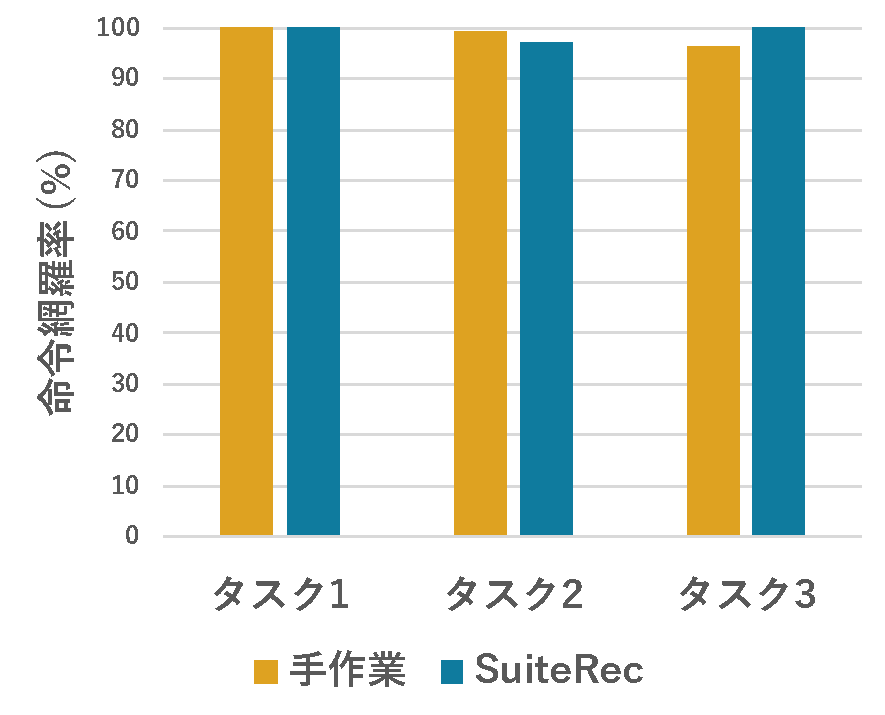
\includegraphics[width=9cm]{pic/C0.pdf}
  \caption{命令網羅の平均カバレッジ}
  \label{C0}
  \end{center}
\end{figure}

\begin{figure}[htbp]
  \begin{center}
   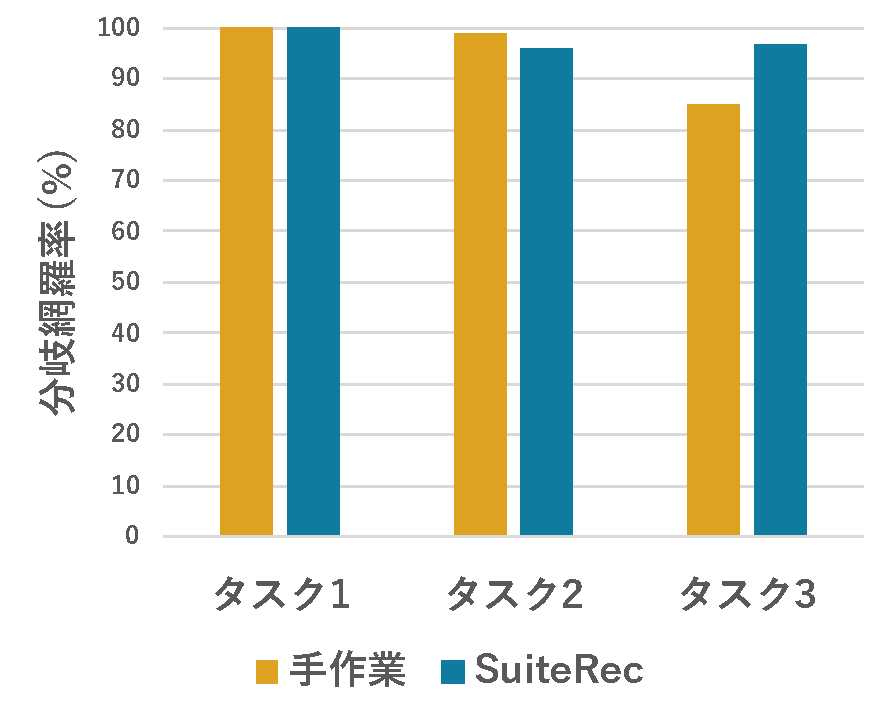
\includegraphics[width=9cm]{pic/C1.pdf}
  \caption{分岐網羅の平均カバレッジ}
  \label{C1}
  \end{center}
\end{figure}


\begin{breakbox}
\textit{条件分岐が多く複雑なプログラムのテストコードを作成する際,{\sf SuiteRec}の利用はカバレッジ(C1)を向上するのに役立つ可能性がある.}
\end{breakbox}

\paragraph{RQ2: {\sf SuiteRec}はテストコードの作成時間を削減できるか?}RQ2では,{\sf SuiteRec}を使用した場合とそうでない場合で被験者のテストコード作成タスクが完了するまでに費やした時間を比較する.図\ref{time}の結果を見ると,3つのタスクの内2つのタスクで{\sf SuiteRec}を使用した場合は,そうでない場合と比べてテスト作成時間が大きくなっていることが分かる.この結果は{\sf SuiteRec}によって推薦される複数のテストスイートを読み理解するのに時間がかかる可能性がある.被験者はほとんどの場合,推薦されるテストコードをそのままの形で再利用することができない.入力したコード片と検出された類似コード片の差分を確認し,テストコードを書き換える必要がある.一方で,タスク2については,{\sf SuiteRec}を利用した場合の方がテスト作成時間が短いことが分かる.我々は,提出されたテストコード調査したところ,カバレッジに差はないものの{\sf SuiteRec}を使用しない場合は,テストケースの重複が多くなっていることが分かった.この結果は,被験者は無駄なテストケースを多く記述するのに時間を費やした可能性がある.


\begin{figure}[htbp]
  \begin{center}
   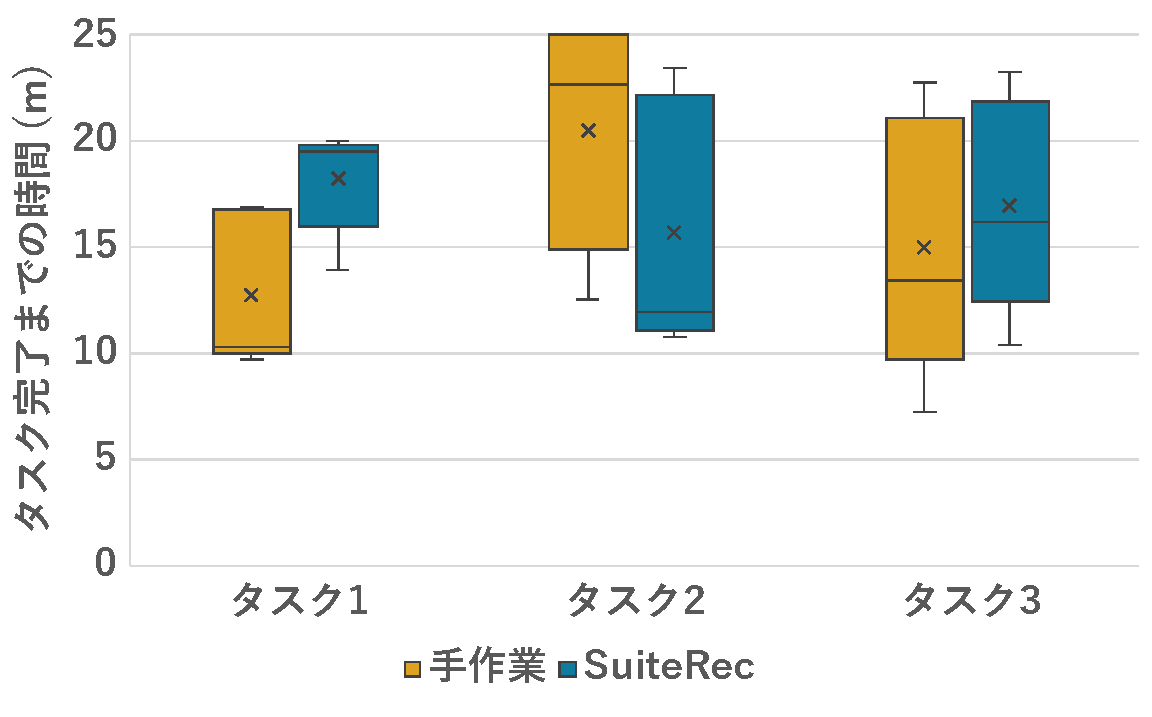
\includegraphics[width=12cm]{pic/time.pdf}
  \caption{テストコード作成タスク終了までの時間}
  \label{time}
  \end{center}
\end{figure}

\begin{breakbox}
\textit{{\sf SuiteRec}の利用は,推薦されたテストスイートを理解し変更する必要があるので,開発者はテストコード作成に多くの時間を費やす可能性がある.}
\end{breakbox}



\paragraph{RQ3: {\sf SuiteRec}は,テストスメルの数が少ないテストコードの作成を支援できるか?}RQ3では,{\sf SuiteRec}を使用した場合とそうでない場合で被験者が作成したテストコード内に含まれるテストスメルの数を比較する.図\ref{smell}の結果は,すべての被験者が提出したテストコード内に含まれていたテストスメルの数の合計を示す.すべてのタスクに対して,{\sf SuiteRec}を使用して作成されたテストコードは,テストスメルをあまり含んでいないことが分かる.この結果は,{\sf SuiteRec}によって推薦されるテストコード自体の品質が高く,被験者はそれを再利用することで品質を維持したままテストコードを作成できたと考えられる.また,{\sf SuiteRec}の出力画面で推薦されるテストスイート内に含まれているテストスメルを提示することで,それを基にテストコードを書き替えることができ,品質が高いテストコードを提出した可能性が考えられる.一方で,{\sf SuiteRec}を使用しなかった場合は,使用した場合と比べ全体として5倍以上,被験者はテストスメルを埋め込んでいた.その中でも多く埋め込まれていたテストスメルとして,``Assertion Roulette'', ``Default Test'',``Eager Test''が挙げられる.多くの被験者は,初期状態のテストメソッドの名前を変更せず,一つのテストメソッド内でコピーアンドペーストによってassert文を記述していたのが原因だと考えられる.実際に,既存研究でもこれらのテストスメルが,既存プロジェクトで多く検出されていることが報告されている\cite{Peruma}.

\begin{figure}[htbp]
  \begin{center}
   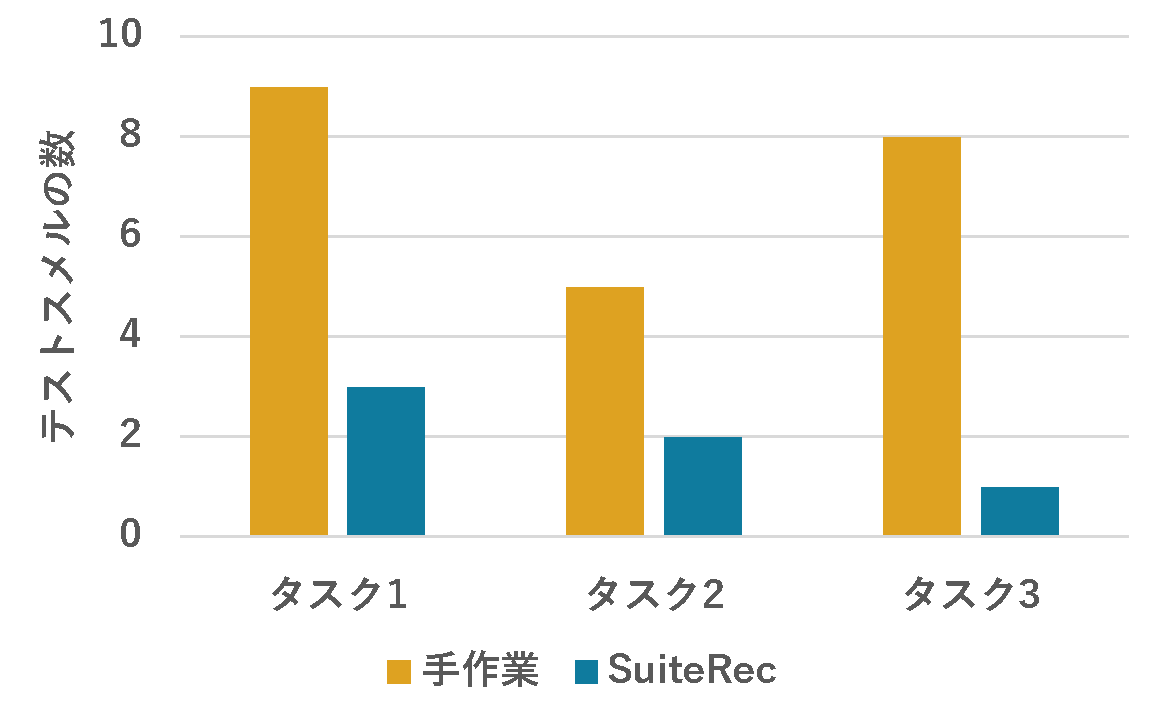
\includegraphics[width=12cm]{pic/smells.pdf}
  \caption{テストコード内に含まれていたテストスメルの数}
  \label{smell}
  \end{center}
\end{figure}


\vspace{\baselineskip}

\begin{breakbox}
\textit{開発者は,{\sf SuiteRec}によって推薦される高品質のテストスイートを参考にすることで品質の高いテストコードを作成できる可能性がある.}
\end{breakbox}

\paragraph{RQ4: {\sf SuiteRec}の利用は,開発者のテストコード作成タスクの認識にどう影響するか?}

RQ4では,評価実験の後,被験者に対して実験タスクに関するアンケートを実施した.図\ref{QA}は実施したアンケートの内容とその結果を示す.初めの2つの質問から,被験者は,実験タスクを明確に理解し(質問1),実験タスクを終えるのに十分な時間があったことが分かる(質問2).残りの質問については,{\sf SuiteRec}を使用した場合とそうでない場合で,実験タスクに対する意見に違いがある.

質問3の回答から被験者は,テストコードを作成する際に,{\sf SuiteRec}を用いるとテストコード作成を容易に感じることができる.しかし,この結果は実際のタスクの完了までの時間(図\ref{time})とは対照的であり,{\sf SuiteRec}を使用した場合の方がタスクの完了までにかかる時間が長いことが分かる.被験者は,推薦された複数のテストスイートを読み理解して再利用するかどうかを決定する.また,テストコードはそのままの状態で適用することはできず,入力コードと検出された類似コードの差分を理解し,テストコードに適切な修正を加える必要がある.我々は,{\sf SuiteRec}を使用した場合,被験者はこの部分に多くの時間を費やすことがあると推測している.しかし,これらの作業は単純で繰り返すことが多いので被験者は容易に感じた可能性がある.また,推薦されたテストコードがテスト項目を考える上で参考になり,テストコードの記述には時間がかかるが全体としては容易な作業だと感じた可能性が高い.

質問4の回答から被験者は,{\sf SuiteRec}を使用した場合,自身で作成したテストコードのカバレッジに自信があることが分かる.一方で,何も使用しなかった場合40\%の被験者がネガティブな回答を報告した.しかし,実際に提出されたテストコードのカバレッジには,ほとんど差がないことが分かる(図\ref{C0},\ref{C1}).開発者が自分自身で作成したテストコードのカバレッジに自信を持つことは重要である.開発者は,自分の書いたコードに責任を持ち,不安なくソフトウェアをユーザに提供できることは,ソフトウェアテストを行う目的の一つである.

質問5の回答から,何も使わずテストコードを作成した場合,40\%の被験者が自身の書いたテストコードの品質に自信が持てないことが分かった.実際に,提出されたテストコード内のテストスメルの数も{\sf SuiteRec}を使用した場合よりも多く存在していることが分かる(図\ref{smell}).開発者は無意識の内にテストスメルを埋め込み,それが後の保守活動を困難にする.{\sf SuiteRec}の利用は,開発者にテストコードの品質に対する意識を与えることでテストメルの数を減らし,作成したコードに自信をもたらす.一方で,{\sf SuiteRec}を利用した場合でも品質に関してネガティブな意見も存在した.アンケートの記述項目では,テストスメルの存在は意識できたが具体的にどう修正して無くすことができるのか分からなかったと報告されていた.これは{\sf SuiteRec}の更なる改善の必要性を示しており,各テストスメルに対するリファクタリング方法も提示する機能を追加すべきだと考えている.

\begin{figure}[htbp]
  \begin{center}
   \includegraphics[width=15cm]{pic/suiterec-expt.pdf}
  \caption{実験後のアンケートの回答}
  \label{QA}
  \end{center}
\end{figure}

\begin{breakbox}
\textit{{\sf SuiteRec}を利用した場合,開発者はテスト作成タスクを容易だと認識し,作成したテストコードに自信が持てる.}
\end{breakbox}

\subsection{評価実験2: 推薦されるテストスイートの順位付けに関する実験}
評価実験2では,{\sf SuiteRec}によって推薦される複数のテストスイートの順位付けの妥当性について検証する.我々は,被験者の数を増やすためにオンライン上で行うアンケートを実施した.被験者は,{\sf SuiteRec}によって1位から10位まで順位付けられたテストスイートを読み,推薦されたテストスイートを参考にしたいかどうかを選択する.被験者のアンケート結果を基に,以下のリサーチクエスチョンに答えることを目指す.

\begin{description}
\item[RQ5: SuiteRecは開発者が参考したいテストスイートを上位に推薦できるか?]
アンケート調査で,被験者が参考にしたいと回答したテストスイートが実際の{\sf SuiteRec}の出力結果で上位に推薦されているかを評価する.評価方法では,検索エンジンなどの評価で用いられる代表的な評価指標を利用した.
\end{description}

以降,4.2.1節では,評価実験2で用いた実験用データセットについて説明する.4.2.2節では,評価実験1の手順について説明する.最後に4.2.3節で,評価実験2の結果について説明する.

\subsubsection{評価実験2のデータセット}

評価実験2を実施するために,{\sf SuiteRec}によって推薦されるテストスイートの順位付けに関するアンケート調査を実施した.我々は被験者の数を増やすためにオンライン上で行えるアンケートを作成した.その結果,学生11人と社会人3人の計14人の被験者がアンケートに回答した.アンケートのパーソナリティに関する項目によると,9割以上の被験者が2年以上のプログラミング経験があり,6割以上の被験者が2年以上のJavaの経験があった.また,すべての被験者が授業などの講義でソフトウェアテストに関する基本的な知識を持っていた.

評価実験2では,被験者に2つのタスクを割り当てた.以降,これらの2つのタスクをタスクA,タスクBと呼ぶ.被験者は,各タスクで与えられる関数単位のプロダクションコードのテストコードを作成する際に,{\sf SuiteRec}によって推薦されるテストスイートが参考になるかどうかを選択する.以下に,各タスクの概要を示す.

\begin{description}
\item[タスクA]~\\
タスクAは,会計処理を行うプログラムであり,ユーザが購入したアイテムの合計金額を計算するJavaメソッドである.以下に,タスクAのプロダクションコードの仕様とソースコードを示す.
\begin{itembox}[l]{タスクAのプロダクションコードの仕様}
\begin{itemize}
\item 入力配列 item[ ]の要素の合計値を返す.
\item 入力配列の要素数が0の時,$-1$を返す.
\item 引数:整数型の配列 item[ ]
\item 返り値:配列要素の合計値 totalprice
\end{itemize}
\end{itembox}

\begin{figure}[htbp]
  \begin{center}
    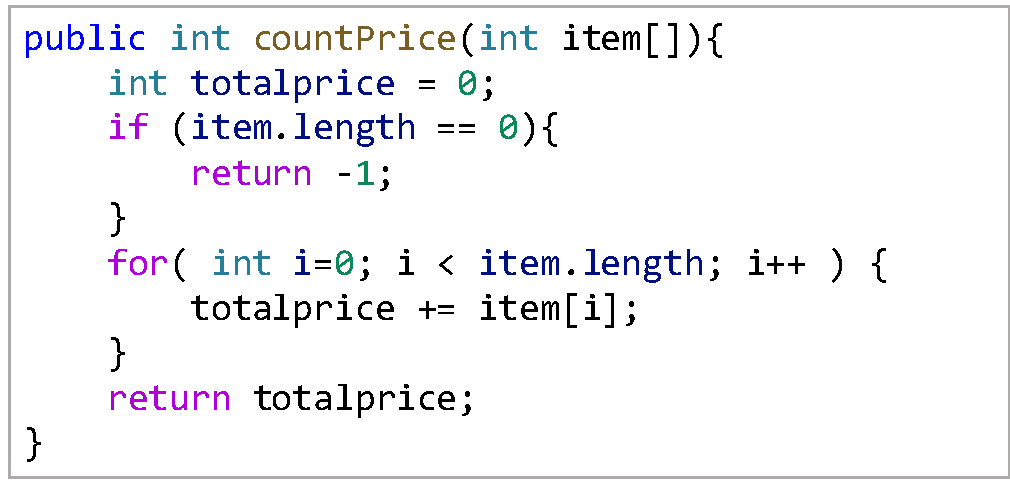
\includegraphics[clip,width=12cm]{taskA.pdf}
    \caption{タスクAのプロダクションコード}
    \label{E1}
  \end{center}
\end{figure}

\item[タスクB]~\\
タスクBは,10進数を2進数または,16進数に変換するプログラムである.第1引数に応じて,第2引数の数値の変換方法を変更し結果を出力するJavaメソッドである.以下に,タスクBのプロダクションコードの仕様とソースコードを示す.


\begin{itembox}[l]{タスクBのプロダクションコードの仕様}
\begin{itemize}
\item 第1引数が ``bin'' の場合,第2引数(10進数)を2進数に変換する.
\item 第1引数が ``hex''の場合,第2引数(10進数)を16進数に変換する.
\item 第1引数が上記以外の場合,``can not conversion''を返す.
\end{itemize}
\end{itembox}

\begin{figure}[htbp]
  \begin{center}
    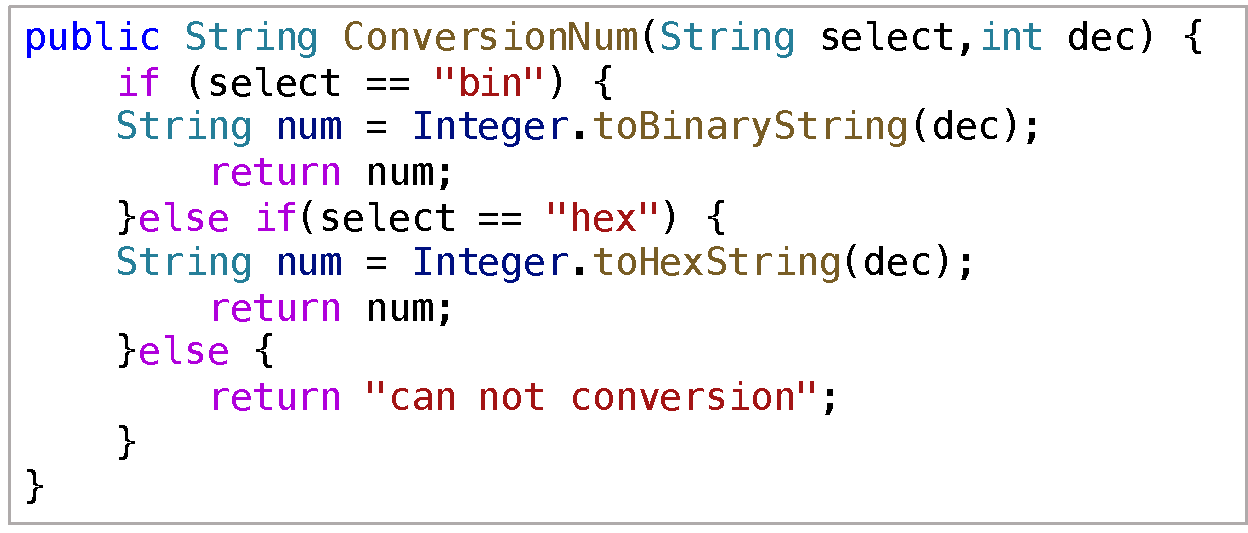
\includegraphics[clip,width=12cm]{taskB.pdf}
    \caption{タスクBのプロダクションコード}
    \label{E2}
  \end{center}
\end{figure}

\end{description}

\subsubsection{評価実験2の手順}

5.1節で説明した,実験タスクを用いた評価実験2の手順について説明する.評価実験2は,Google Formを用いたオンライン上のアンケートで実施された.アンケートでは,最初に被験者間の事前知識の違いによる結果の相違をなくすために,ソフトウェアテストに関する基本的な資料と良いテストコードの設計に関する資料を提供した.また,アンケートの回答をする際には事前資料を参考にしながら回答することを推奨した.その後,被験者に2つの実験タスクから推薦される合計20個のテストスイートについて参考にしたいかどうかを選択してもらった.また,被験者には,なぜその回答を選択したのか,その理由を代表的な悪いテストコードの設計の選択肢から回答してもらった(自由回答).最後に,実験タスク終了後に,被験者のパーソナリティに関するアンケートに回答してもらった.

\subsubsection{評価実験2の結果}

本節では,{\sf SuiteRec}によって推薦されるテストスイートの順位付けに関する評価実験の結果を報告する.そして,4.2節で説明したリサーチクエスチョン5について,実験結果を基に回答する.

\paragraph{RQ5: SuiteRecは,開発者が参考にしたいテストスイートを上位に推薦できるか?}
RQ5では,15人の被験者によるアンケート結果を代表的な3つのランキングの評価指標に基づいて計算する.以下に,評価実験2で利用した評価指標について説明する.


\begin{description}
\item[Mean Reciprocal Rank (MRR)]~\\
MRRは,推薦リストを上位から確認し,最初に適合した要素の順位を計算に利用したランキング指標である.MRRは,0から1の値をとり,すべてのユーザに対して推薦リストの第1番目のアイテムが適合アイテムならば,1になる.一方で,正解が一つもリストに含まれない場合は,0になる.この指標の特徴として,ランキング上位での順位の差異は指標に大きく影響するが,下位での順位の差異はあまり影響を与えない.

\[
  MRR =
  \frac{1}{|U|}\sum_{u\in U} \frac{1}{k_u}
\]
\begin{itemize}
\item $uは各対象ユーザ,Uは全対象ユーザ$
\item $k_uはユーザuへの推薦リストのうち,最初にuが適合するアイテムが出現した順位$
\end{itemize}


\item[Mean Average Precision(MAP)]~\\
MAPは,AP(Average Precision)の値を対象のユーザ数で平均した値である.APとは,適合アイテムが出現した時点をそれぞれ閾値として,閾値ごとのPrecisionを算出し,Precisionを平均した値である.以下にAPとMAPの式を示す.

\[
  AP(u) =
  \sum_{k=1}^{N} \frac{Precision@k \cdot y_k}{\sum_{i=1}^{k}y_i}
\]

\[
  y_k = \begin{cases}
    1 : 上位k番目が適合アイテム \\
    0 : それ以外
  \end{cases}
\]

\[
  MAP =
  \frac{1}{|U|}\sum_{u\in U} AP(u)
\]
\begin{itemize}
\item $uは各対象ユーザ,Uは全対象ユーザ$
\end{itemize}


\item[Mean Precision@N (MP@N)]~\\
MP@Nは,推薦ランキングの上位N番目のPrecision@Nを平均した値である.Precision@Nとは,上位N番目までのユーザが実際に適合したアイテムの内,推薦リストでどれだけカバーできたかの割合である.以下に上位k番目のPrecision@NとMP@Nの式を示す.

\[
  Precision@N =
  \frac{|a \cap p_N|}{N}
\]
\begin{itemize}
\item $N:考慮する上位ランキングの数$
\item $a:ユーザが適合したアイテム集合$
\item $p_N:TopNの推薦リスト$
\end{itemize}

\[
  MP@N =
  \frac{1}{|U|}\sum_{u\in U} Precision@N(u)
\]
\begin{itemize}
\item $uは各対象ユーザ,Uは全対象ユーザ$
\end{itemize}

\end{description}



\begin{comment}
\item[Mean Recall@N (MR@N)]~\\
MR@Nは,推薦ランキングの上位N番目のRecallを平均した値である.Recall@Nとは,ユーザが実際に適合した上位N番目までのアイテムのうち,推薦リストでどれだけカバーできたかの割合である.以下に上位k番目のRecall@NとMR@Nの式を示す.

\[
  Recall@N =
  \frac{|a \cap p_N|}{|a|}
\]
\begin{itemize}
\item $N:考慮する上位ランキングの数$
\item $a:ユーザが適合したアイテム集合$
\item $p_N:TopNの推薦リスト$
\end{itemize}

\[
  MR@N =
  \frac{1}{|U|}\sum_{u\in U} Recall@N(u)
\]
\begin{itemize}
\item $uは各対象ユーザ,Uは全対象ユーザ$
\end{itemize}

\end{description}
\end{comment}

\begin{table}[h]
\caption{MAPとMRRの評価結果}
\label{map}
\begin{center}
\begin{tabular}{|p{3cm}|p{3cm}|p{3cm}|}
\hline \hline
\multicolumn{1}{|r|}{} & \multicolumn{1}{p{3cm}|}{MAP} & \multicolumn{1}{p{3cm}|}{MRR} \\ \hline
タスクA & \multicolumn{1}{r|}{84.1\%} & \multicolumn{1}{r|}{83.3\%} \\ \hline
タスクB & \multicolumn{1}{r|}{98.3\%} & \multicolumn{1}{r|}{100\%} \\ \hline
合計 & \multicolumn{1}{r|}{91.2\%} & \multicolumn{1}{r|}{94.1\%} \\ \hline
\end{tabular}
\end{center}
\end{table}


\begin{comment}
\begin{table}[h]
\caption{MR@Nの評価結果}
\label{pre}
\begin{center}
\begin{tabular}{|p{3cm}|p{2cm}|p{2cm}|p{2cm}|p{2cm}|}
\hline \hline
Recall-topK & top1 & top3 & top5 & top10 \\ \hline
タスクA & \multicolumn{1}{r|}{14.2\%} & \multicolumn{1}{r|}{50.9\%} & \multicolumn{1}{r|}{89.2\%} & \multicolumn{1}{r|}{93.3\%} \\ \hline
タスクB & \multicolumn{1}{r|}{20.3\%} & \multicolumn{1}{r|}{58.8\%} & \multicolumn{1}{r|}{92.3\%} & \multicolumn{1}{r|}{100\%} \\ \hline
合計 & \multicolumn{1}{r|}{17.3\%} & \multicolumn{1}{r|}{54.8\%} & \multicolumn{1}{r|}{90.7\%} & \multicolumn{1}{r|}{96.7\%} \\ \hline
\end{tabular}
\end{center}
\end{table}
\end{comment}


\begin{table}[h]
\caption{MP@Nの評価結果}
\label{pre}
\begin{center}
\begin{tabular}{|p{3cm}|p{2cm}|p{2cm}|p{2cm}|p{2cm}|}
\hline \hline
Precision-topN & top1 & top3 & top5 & top10 \\ \hline
タスクA & \multicolumn{1}{r|}{73.3\%} & \multicolumn{1}{r|}{82.2\%} & \multicolumn{1}{r|}{85.3\%} & \multicolumn{1}{r|}{45.3\%} \\ \hline
タスクB & \multicolumn{1}{r|}{100\%} & \multicolumn{1}{r|}{97.8\%} & \multicolumn{1}{r|}{93.3\%} & \multicolumn{1}{r|}{53.3\%} \\ \hline
合計 & \multicolumn{1}{r|}{86.7\%} & \multicolumn{1}{r|}{90.0\%} & \multicolumn{1}{r|}{89.3\%} & \multicolumn{1}{r|}{49.3\%} \\ \hline
\end{tabular}
\end{center}
\end{table}


上記の評価指標を基に計算した結果を表\ref{map},\ref{pre}に示す.

表3は,MAPとMRRの評価結果を示す.実験の対象とした2つのタスクに対してMAPは80\%を超えており,高精度で開発者が参考にしたいテストスイートをランキングの上位に推薦できることが分かった.また,MRRについても各タスクに対して80\%の超えている.一般的に,開発者はランキングの上位に表示されるテストスイートを参考にしやすいことを考えると,上位の含まれる適合アイテムの数が大きく影響するMRRの結果が高いことは,重要である.表4は,MP@Kの評価結果を示す.各タスクにおいて,top3の精度は80\%を超えており{\sf SuiteRec}は,ランキングの上位3位までに開発者が参考にしたいテストスイートを高精度で出力することができた.

各タスク毎の結果を比較すると,MAP,MRR,MP@Nの3つの結果についてタスクAはタスクBよりも低いことが分かる.これはタスクAについて{\sf SuiteRec}が上位に推薦するテストコード内に含まれるテストスメルが関係していると考えられる.すなわち,{\sf SuiteRec}のランキング手法は類似度を優先するためテストスメルを多く含むテストスイートであっても,そのテストスイートに対応する類似コード片の類似度が高い場合,テストスイートは上位に推薦される.今回,タスクAについて{\sf SuiteRec}が上位に推薦したテストスイートは,類似度は高かったがテストスメルを含んでいた.従って,被験者の中には,上位で推薦されたテストスイートを参考にしたいと思わない被験者も存在した.一方で,タスクBについてはMRRとMP@Nの結果から分かるように,{\sf SuiteRec}によって上位に推薦されたテストスイートがテストスメルが少なく,類似度が高いことが分かる.このような場合,{\sf SuiteRec}は高い精度で開発者が参考にしたいテストスイートを上位に推薦できる.今後は,{\sf SuiteRec}のランキングについて,再利用しやすい類似度を優先とした並び替えと品質を重視したテストスメルの数を優先とした並び替えを開発者の好みによって選択できるように,ランキング手法を拡張する必要がある.

\vspace{\baselineskip}

\begin{breakbox}
\textit{{\sf SuiteRec}は,開発者が参考にしたいテストスイートを高精度でランキングの上位に推薦できる.}
\end{breakbox}


\newpage
\section{議論}

本章では,4章の評価実験の結果から{\sf SuiteRec}の有用性及び妥当性への脅威について議論する.

\subsection{SuiteRecの有用性}
本節では,4章の評価実験の結果を基に{\sf SuiteRec}の有用性について考察する.RQ1では,作成したテストコードのカバレッジを測定した.被験者が実施したテストコード作成タスクにおいて,比較的単純な構造のプロダクションコード(タスク1,タスク2)のテストを作成する場合,{\sf SuiteRec}の利用の有無でカバレッジ(C0,C1)にほとんど差がないことは重要な実験結果である.{\sf SuiteRec}を使用した場合,テストコード作成に多くの時間を費やす可能性がある(RQ2)ことを考慮すれば,何も使用せずにテストコードを作成した方が開発時間を節約することができる.一方で,分岐数が多く複雑なプログラムのテストを作成する際,{\sf SuiteRec}の利用はカバレッジ(C1)を10\%以上向上できることが分かった.この結果は,推薦されたテストスイートは開発者がテスト項目を考える上で有益な情報になったと考えられる.実際に,実験後のアンケートの回答はこの考察を裏付けている.{\sf SuiteRec}を利用した場合,すべての開発者は自身が作成したテストコードのカバレッジに自信があると回答した(質問4).また,アンケートの自由記述欄の回答では,ある被験者は「テスト項目を推薦されたテストコードを見て,見落としていたテスト項目に気づくことができた」と回答した.これらの結果の有意性を検討するには被験者を増やした更なる調査が必要であり,開発者のテストコード作成スキルや経験に依存すると考えられる.

RQ3は,{\sf SuiteRec}を使用して作成したテストコードはテストスメルの数が少なく品質が高いことを示した.開発者によって無意識に埋め込まれるテストスメルの存在は,後の保守活動を困難にする.{\sf SuiteRec}はテストスメルの存在を被験者に意識させることで,保守性の高いテストコードの作成を支援できる可能性がある.実際にアンケートの自由記述欄の回答には「提示されたテストスメルを理解し,それをなくすようにリファクタリングしテストコードを作成した」という報告がされている.さらに,「メソッド名を考える際に推薦されたテストコードのテストメソッド名が参考になった」という可読性向上に有益だったという回答も存在した.一方で,回答の中には「テストスメルの存在は意識できたが具体的にどう修正して無くすことができるのか分からなかった」という回答も存在した.これは{\sf SuiteRec}の更なる改善の必要性を示しており,各テストスメルに対するリファクタリング方法も提示すべきだと考えている.

RQ5は,{\sf SuiteRec}は開発者が参考にしたいテストスイートを出力結果の上位に推薦できることを示した.{\sf SuiteRec}のランキング手法では,類似度とテストスメルの数の2つの要素に基づいて順位付けされており,再利用しやすく品質の高いテストコードをランキングの上位に提示する.RQ3の結果を考慮すると{\sf SuiteRec}の出力結果の上位に推薦されるテストスイートを参考にすることで,開発者は高品質のテストコードを作成できる可能性がある.

\subsection{妥当性への脅威}

本節では,提案ツール{\sf SuiteRec}と評価実験における妥当性の脅威を説明する.

{\sf SuiteRec}は,入力コード片に対応する類似コード片をOSSプロジェクトから検索し,その類似コード片に対応するテストスイートを推薦する.そのため,入力コード片の類似コード片が見つからないとテストスイートを推薦できない.また,類似コード片を検出できたとしても類似度が低い場合,推薦されるテストスイートは参考にならない可能性がある.{\sf NiCad}が検出するコードクローンはタイプ2,3でありタイプ3のような命令文の挿入・削除が複数存在するような類似コード片は振る舞いが異なる場合がある.このような場合は,テストコードを再利用することは困難であり,推薦できるテストスイートは狭い範囲に限定される可能性がある.

{\sf SuiteRec}で利用した{\sf Nicad}は,検索対象のプロジェクトに対して一度に検索できるサイズに制限がある.従って,検索対象が大規模なプロジェクトになると計算コストが高い.しかし,{\sf Nicad}の代わりに{\sf SourcererCC}\cite{SourcererCC}や{\sf FaCoY}\cite{FaCoY}などのコード検索エンジンを使用すれば,大規模なプロジェクトに対しても一度の処理で検索することが可能である.本研究では,テストコードの再利用性を考慮し類似度の高いコード片を検出できる{\sf Nicad}を使用した.また,検出時間を短縮化するために検索処理を並列化するように{\sf SuiteRec}に実装した.今後は,{\sf SuiteRec}を他のコードクローン検出ツールにも対応させ,テストコードを推薦するまでの時間および推薦されたテストコードの違いを確認する必要がある.

{\sf SuiteRec}の評価では,被験者による実験を行い{\sf SuiteRec}を利用した場合とそうでない場合で作成されたテストコードを比較することで,有用性を示している.そのため,被験者のプログラミングスキルやテストコードの作成経験が実験結果に影響を与える可能性がある.ただし,アンケートのパーソナリティに関する項目によると9割の被験者が2年以上のプログラミング経験があり,その内8割の被験者が単体テストの作成経験があると回答した.また,実験前にソフトウェアテストに関する講義と練習問題を実施しており,被験者による本実験への影響は少ないと考えられる.一方で,評価実験1では3つの実験タスクを使用したが,今回の結果が使用された実験タスクに限定される可能性がある.評価実験1では,被験者がテスト対象のプロダクションコードの仕様を十分理解していることが前提となるので,競技プログラミングで用いられるコードを利用した.しかし,これが実際のソフトウェアプロジェクトで使用されるプロダクションコードの場合結果が変わる可能性がある.今後,OSSプロジェクトの実用コード片に対して実験を行い,結果がどのように変化するのか確認する必要がある.

評価実験2では,被験者を多くするためにオンライン上のアンケートで実験を実施した.評価実験2を実施した15人の被験者の内,9人は評価実験1も実施している.そのため,評価実験1の背景知識が評価実験2に影響した可能性がある.今後は,評価実験1を実施してない被験者の数をさらに増加させ一般性を示す必要がある.




\newpage
\section{関連研究}
本章では,提案ツール{\sf SuiteRec}の基本となるアイディアであるクローンペア間でのテストコード再利用に関する既存研究を紹介する.

Zhangら\cite{Zhang2017}はクローンペア間でコードを移植を行い,移植前と移植後のテスト結果を比較しその情報を基に既存テストコードを再利用するツール{\sf Grafter}を提案した.有名OSSプロジェクトを対象とした{\sf Grafter}の評価実験では,コードクローン検出ツール{\sf DECKARD}\cite{Jiang2007}によって検出されたどちらか片方のコード片テストコードが存在するクローンペア52個の内94\%でコード移植に成功し,テストコードを再利用できることを示した.

Sohaら\cite{skipper}は,コード片を再利用する時にそのコード片に対応するテストスイートの関連部分を半自動で再利用および変換を行うツール{ \sf Skipper}を提案した.{ \sf Skipper}のアプローチは,再利用元のコード片のテストスイートを動的解析し,どのテストケースが再利用先のコード片を実行するかを特定する.そして,コード片の再利用タスクを支援するツール{\sf Gilligan}\cite{gilligan10,gilligan34}に基づいて,テストスイートを変換し再利用する.{ \sf Skipper}の変換プロセスでは,開発者が変換プロセスを導くための詳細な再利用計画を決める必要がある.被験者による{ \sf Skipper}の評価実験では,被験者の手作業でのテスト作成タスクと比較して,テスト作成時間の短縮化できカバレッジが向上したことを示した.

{\sf SuiteRec}はこれらのツールとは,2つの視点で異なる.1つ目は,{\sf SuiteRec}はOSS上のリポジトリから類似コード検索する.大規模なソースコードリポジトリ内で検索をかけることで,多くのテストスイートを見つけることができる可能性がある.次に,{\sf SuiteRec}はテストスイートを推薦するだけであり,クローンペア間の詳細なテスト再利用計画は開発者に委ねていること.たとえ,自動的にテストを再利用できたとしても品質の低いコードを拡散することは,後の保守活動を困難にさせる.テストスメルを提示し,開発者自身にリファクタリングさせることで作成したテストに自信が持てると考える.

\newpage
\section{まとめと今後の課題}
本研究では,コードクローン検出技術を用いたテストコード自動推薦ツール{\sf SuiteRec}を提案した.{\sf SuiteRec}は,開発者から入力された関数単位のコード片に対して類似コード片を検出し,その類似コード片に対応するテストスイートを推薦する.さらに,テストコードの良くない実装を表す指標であるテストスメルを開発者に提示し,より品質の高いテストスイートを推薦できるように推薦順位がランキングされる.{\sf SuiteRec}の評価では,被験者によって{\sf SuiteRec}の使用した場合とそうでない場合でテストコードの作成してもらい,テスト作成をどの程度支援できるかを定量的および定性的に評価した.その結果,{\sf SuiteRec}の利用は条件分岐が多く複雑なプログラムのテストコードを作成する際にコードカバレッジの向上に効果的であること,作成したテストコードの内のテストスメルの数が少なく品質が高いことが分かった.また,{\sf SuiteRec}は開発者が参考にしたテストスイートを上位に推薦できることを確認した.実験後のアンケートによる定性的な評価では,{\sf SuiteRec}を使用した場合被験者はテストコードの作成が容易になると認識し,また自分の作成したコードに自信が持てることが分かった.

今後の課題として,以下が挙げられる.

\begin{itemize}
\item より実践的な利用に備えてツールを改善する必要がある.具体的には,{\sf SuiteRec}に推薦されるテストコードを自動編集できる機能とテストスメルに対するリファクタリング方法を提示する機能を追加する予定である.
\item {\sf SuiteRec}の有意差を測るために評価実験1では,被験者を増やした更なる実験が必要である.また,経験値による効果の影響をなくすために対象の被験者を学生だけでなくテストコード作成経験の豊富なエンジニアに対しても参加してもらう必要がある.
\item {\sf SuiteRec}で採用したコードクローン検出ツール{\sf NiCad}だけでは,検出できるコードクローンの数に限りがある.検出できるコードクローンの幅を広げるために{\sf SuiteRec}を複数のコードクローン検出ツールに対応できるようにし,より多くテストスイートを推薦できるようにする必要がある.
\end{itemize}


%
% 謝辞
%
\acknowledgements

本研究を進めるにあたり,多くの方々に御指導及び御助言頂きました.ここに謝意を添えて御名前を記させて頂きます.

奈良先端科学技術大学院大学先端科学技術研究科情報科学領域 飯田 元 教授には,ご多忙にも関わらず,毎週の進捗報告ミーティングや論文輪講に御参加して頂き,その中で常に本質的な御指導及び御助言を頂きました.また,本研究に限らず,GEIOTやenPiTなど学外のプログラムに参加させていただき2年間充実した大学院生活を送ることができたことは,先生の御指導と御人柄によるものと確信しております.心より深く感謝を申し上げます.

奈良先端科学技術大学院大学先端科学技術研究科情報科学領域 市川 昊平 准教授には,毎週の進捗報告ミーティングや論文輪講を通して,本研究に関して常に適切な御指導及び御助言を頂きました.また,本研究に限らず,enPiTプログラムの参加やタイ留学など大変貴重な経験をさせて頂き,充実した大学院生活を送ることができました.心より深く感謝を申し上げます.

京都工芸繊維大学情報工学課程 崔恩 瀞 助教には,本研究を進めるにあたって,積極的に打ち合わせや連絡を取って頂き,その中で終始適切な御指導及び御助言を頂きました.さらに,京都工芸繊維大学に移転した後も論文投稿時や論文輪講に関して常に適切な御助言をして頂き,研究室に配属されてから 2年間,大変お世話になりました.また,本研究に限らず就職活動などでも助言を頂いたことや積極的に学生に関わって頂き,充実した生活を送ることができたことは,先生の御指導と御人柄によるものと確信しております.心より深く感謝を申し上げます.

奈良先端科学技術大学院大学先端科学技術研究科情報科学領域 高橋 慧智 助教には,本研究の方向性や問題点などに関して,多くのご意見を頂きました.また,本研究についてだけではなく,専門知識に関して様々なご教授を頂き,ソフトウェア工学に止まらず多くのことを学ばさせて頂きました.本論文ならびに研究生活において,常に多くのご意見を賜りました心から御礼申し上げます.
 
最後に,その他様々な御指導及び御助言等を頂いた奈良先端科学技術大学院大学先端科学技術研究科情報科学領域ソフトウェア設計学研究室・超高信頼ソフトウェアシステム検証学研究室の皆様に深く感謝いたします.


%
% 参考文献
% ここでは \reference を使って、自分でリストを作るか、BibTeX を使って
% リストをつくって下さい。この例では BibTeX を作るような形式になってい
% ます。
%
\newpage
%\reference
\bibliographystyle{plain}
\bibliography{mthesis}
%
% 付録
%
\appendix

\section{おまけその1}
\label{omake1}



\begin{figure}
\centerline{これはおまけの図です。}
\caption{おまけの図}
\end{figure}


\section{おまけその2}



\end{document}

